%\documentclass[twocolumn,prc,showpacs,nofootinbib,preprintnumbers,amsmath,amssymb,superscriptaddress]{revtex4-1}
\documentclass[11pt,preprint,tightenlines,
showpacs,preprintnumbers,amsmath,amssymb,superscriptaddress,a4paper,nofootinbib]{revtex4-1}

\usepackage{nicefrac}
%\usepackage{times}
\usepackage{natbib}
\usepackage{amssymb,amsbsy,amsmath,amsfonts}
\usepackage{graphicx}% Include figure files
\usepackage{epsf,epsfig,float,latexsym,amsthm,fancyhdr,rotating}
\usepackage{graphics,psfrag,longtable}
%\usepackage{srcltx}
\usepackage{slashed}
%\usepackage{footnote}
\usepackage[colorlinks,citecolor=blue,linktoc=all,linkcolor=cyan,urlcolor=blue]{hyperref}
\usepackage{upgreek}
 
 \usepackage{setspace}
 
 \renewcommand{\baselinestretch}{1.15}
 
\def\hpm{\hphantom{-}}
\def\beq{\begin{equation}}
\def\eeq{\end{equation}}
\def\bea{\begin{eqnarray}}
\def\eea{\end{eqnarray}}
\def\beqa{\begin{equation}\begin{array}{l}}
\def\eeqa{\end{array}\end{equation}}
% labels
\def\eqlab#1{\label{eq:#1}}
\def\figlab#1{\label{fig:#1}}
\def\tablab#1{\label{tab:#1}}
\def\seclab#1{\label{sec:#1}}
% reference
\def\eref#1{(\ref{eq:#1})}
\def\Eqref#1{Eq.~(\ref{eq:#1})}
\def\figref#1{fig.~\ref{fig:#1}}
\def\fref#1{\ref{fig:#1}}
\def\Figref#1{Fig.~\ref{fig:#1}}
\def\tabref#1{\ref{tab:#1}}
\def\Tabref#1{Table \ref{tab:#1}}
\def\secref#1{Section \ref{sec:#1}}
% vectors
\def\sla#1{#1 \hspace{-2mm} \slash}
\def\slap{p \hspace{-2mm} \slash}
\def\slad{\partial \hspace{-2.2mm} \slash}
\def\slaP{P \!\!\!\! \slash}
% fractions
\def\boxfrac#1#2{\mbox{\small{$\frac{#1}{#2}$}}}
\def\half{\mbox{$\frac{1}{2}$}}
\def\sfrac#1{\mbox{\small{$\frac{1}{#1}$}}}
\def\thalf{\mbox{\small{$\frac{3}{2}$}}}
\def\quarter{\mbox{$\frac{1}{4}$}}
\def\third{\mbox{$\frac{1}{3}$}}
\def\sixth{\mbox{$\frac{1}{6}$}}

% matrices
\def\barr{\left(\begin{array}{c}}
\def\earr{\end{array}\right)}
\def\bmat{\left(\begin{array}{cc}}
\def\emat{\end{array}\right)}
%--------------------------------------------
% symbols
\def\al{\alpha}
\def\be{\beta}
\def\ga{\gamma} \def\Ga{{\it\Gamma}}
\def\de{\delta} \def\De{\Delta}
\def\veps{\varepsilon}  \def\eps{\epsilon}
\def\kp{\kappa}
\def\la{\lambda} \def\La{{\Lambda}}
\def\Pit{{\it\Pi}}
\def\Psit{{\it\Psi}}
\def\si{\sigma} \def\Si{{\it\Sigma}}
\def\th{\theta} \def\vth{\vartheta} \def\Th{\Theta}
\def\w{\omega} \def\W{\Omega} \def\hw{\hat{\omega}}
\def\vfi{\varphi}\def\vphi{\varphi}
\def\z{\zeta}
\def\bra{\langle} \def\ket{\rangle}

\def\pa{\partial}
\def\vrho{\varrho}
\def\barf{\zeta}
\def\ie{{i.e., }}
\def\eg{{e.g.\ }}
\def\cl{\centerline}
\def\ni{\noindent}
\def\pa{\partial}
\def\ra{\rightarrow}
\def\nn{\nonumber}
\def\dd{\mathrm{d}}
\def\cO{\mathcal{O}}
\def\DD{{\mathcal D}}
\def\lag{{\mathcal L}}
\def\ham{{\mathcal H}}
\def\aa{\mathcal{a}}
\def\kk{\mathcal{k}}
%\def\gg{\mathcal{g}}
\def\xx{\mathscr{x}}
\def\yy{\mathscr{y}}
\def\zz{\mathscr{z}}
\def\MM{\mathcal{M}}
\def\MA{{\mathcal A}}
\def\MR{{\mathcal R}}
\def\MQ{{\mathscr q}}
\def\MB{{\mathcal B}}
\def\MP{{\mathcal P}}
\def\TT{{\mathscr T}}
\def\ZZ{\mathcal{Z}}
\def\rZ{\mathantt{Z}}
\def\zZ{\mathpzc{Z}}



\def\bGa{{\bf\Gamma}}
\def\bS{{\bf S}}
\def\psib{\bar{\psi}} \def\Psib{\bar{\Psit}}
\def\pib{\bar{\pi}} \def\Pib{\bar{\Pi}}
\def\xib{\bar{\xi}}

\DeclareMathOperator\arctanh{arctanh}
\DeclareMathOperator\im{Im}
\DeclareMathOperator\re{Re}\def\3d{3-D}
\def\CMS{CMS}
\def\ODI{O$\Delta$I}
\def\ODR{O$\Delta$R}
\newcommand{\lsim}{\, \, \raisebox{-0.8ex}{$\stackrel{\textstyle <}{\sim}$ }}
\def\ol#1{\overline{#1}}
\def\amm{a.m.m.}
%---------------------------------
\def\hate{\hat{\mathbf{e}}}
\def\bq{\mathbf{q}}
\def\bvare{\boldsymbol{\varepsilon}}
\def\bsig{\boldsymbol{\sigma}}


%\textwidth18.5cm
\begin{document}
%\preprint{MITP/13-042}
\title {Moments of unpolarized nucleon structure functions
and the Lamb shift in chiral perturbation theory at next-to-leading order}
\author{Jose Manuel Alarc\'on}
%\affiliation{
%Cluster of Excellence PRISMA Institut f\"ur Kernphysik, Johannes Gutenberg-Universit\"at, Mainz D-55099, Germany}
\affiliation{Departamento de F\'isica Te\'orica \& IPARCOS, Universidad Complutense de Madrid, 28040
Madrid, Spain}
\author{Franziska Hagelstein}
\affiliation{Albert Einstein Center for Fundamental Physics, Institute for Theoretical Physics, University of Bern, Sidlerstrasse 5, CH-3012 Bern, Switzerland}
\author{Vadim Lensky}
\affiliation{Institut f\"ur Kernphysik \&  Cluster of Excellence PRISMA,
 Johannes Gutenberg-Universit\"at  Mainz,  D-55128 Mainz, Germany}
\affiliation{Institute for Theoretical and Experimental Physics, Bol'shaya Cheremushkinskaya 25, 117218 Moscow, Russia}
\affiliation{National Research Nuclear University MEPhI (Moscow Engineering Physics Institute), 115409 Moscow, Russia}
\author{Vladimir Pascalutsa}
\affiliation{Institut f\"ur Kernphysik \&  Cluster of Excellence PRISMA,
 Johannes Gutenberg-Universit\"at  Mainz,  D-55128 Mainz, Germany}
 \email{vladipas@kph.uni-mainz.de}

\begin{abstract}
We obtain predictions of baryon chiral perturbation theory for some of the moments of the nucleon structure functions, related to various polarizabilities, and compare them with the recent Jefferson Lab measurements. 
 the results
for the scalar polarizabilities are new. The latter play an
important role in the calculation of nucleon structure 
effects on the muonic-hydrogen Lamb shift. 
By expanding our results in powers of the inverse nucleon  mass,
we reproduce the known ``heavy-baryon'' expressions. 

\end{abstract}
%\pacs{}
\date{\today}
\maketitle

\tableofcontents

\newpage
\section{Introduction}

Nucleon polarizabilities are accessed in two-photon (Compton) processes,
which in forward kinematics are, through unitarity and analyticity, related to
 moments of inelastic structure functions (see Refs.~\cite{Drechsel:2002ar,Kuhn:2008sy,Hagelstein:2015egb,Pasquini:2018wbl} for review).
This information is used in the extraction of the proton charge radius from
both  elastic electron scattering and atomic spectroscopy, in the form of two-photon-exchange corrections (see Refs.~\cite{Carlson:2007aa,Arrington:2011dn,Afanasev:2017gsk} for review). The interest in the proton polarizabilities has increased since the experimental determination of the proton radius from $\mu$H \cite{Pohl:2010zza,Antognini:1900ns} found a value which initially deviated by $\sim 7\,\sigma$ from the value obtained from normal hydrogen ($e$H) spectroscopy and $ep$ scattering~\cite{Mohr:2012aa}.
 The muon in $\mu$H is orbiting much closer to the proton than the electron in $e$H, making the $\mu$H spectrum be much stronger influenced by the internal electromagnetic structure of the proton. For the Lamb shift, the scalar dipole polarizabilities are of interest, while the planned measurements of the ground-state hyperfine splitting in $\mu$H \cite{Pohl:2016xsr} will bring the spin polarizabilities to the center of attention.



In this work, we consider moments of the nucleon unpolarized structure functions $F_{1}(x, Q^2)$ and $F_{2}(x, Q^2)$.
We focus on the low momentum transfer ($Q^2$) regime, where we employ the framework of chiral effective-field theory up to and including next-to-leading order (NLO). 
We use a manifestly-covariant extension of SU(2) Chiral Perturbation Theory ($\chi$PT) \cite{Weinberg:1978kz,Gasser:1983yg} to the baryon sector \cite{Gasser:1987rb,Gegelia:1999gf,Fuchs:2003qc} --- called Baryon $\chi$PT (B$\chi$PT) --- with explicit 
inclusion of the $\Delta(1232)$-isobar fields in the $\de$-counting scheme
\cite{Pascalutsa:2003aa} (see Ref.~\cite[Sec.~4]{Pascalutsa:2006up} for review).
In this calculation, we only consider the predictive orders, i.e., the ones where no
low-energy constants (LECs) specific to two-photon processes appear. 
Our results are given in terms of well-known parameters,
listed in Table \ref{tab:constants}, obtained from data other than observables of Compton processes or  polarizabilities.
In this sense, our present work continues testing the  ``predictive power''  of $\chi$PT for Compton processes,  as previously done for the static polarizabilities and real Compton scattering (RCS) \cite{Lensky:2009uv, Lensky:2015awa}, 
generalized polarizabilities and virtual Compton scattering (VCS) \cite{Lensky:2016nui},
and the calculation of two-photon-exchange corrections to the \mbox{(muonic-)}hydrogen
Lamb shift \cite{Alarcon:2013cba,Lensky:2017bwi}. All of these studies, 
including the present one, are done in the same framework, using the same set of parameters.

With the present work, we extend our previous results for forward doubly-virtual Compton scattering (VVCS)~\cite{Lensky:2014dda},
including the
Coulomb-quadrupole $(C2)$ $N\to \Delta$ transition \cite{Pascalutsa:2005vq,Pascalutsa:2005ts} (see Appendix \ref{sec:DeltaTreePolarizabilities} for results), producing new results for the scalar polarizabilities.
Upon expanding our results in powers of the inverse nucleon mass, $M_N^{-1}$, we are able to reproduce the LO results
of Heavy-Baryon Chiral Perturbation Theory (HB$\chi$PT) 
which exist for the magnetic polarizability \cite{Birse:2012eb}. 
We, however, do not see a rationale to drop the higher-order $M_N^{-1}$ terms when they are not 
negligible (i.e., when their actual size exceeds by far the natural estimate
for the size of higher-order terms).


 Another approach used in the literature to calculate the polarizabilities in $\chi$PT is the infrared regularization (IR) scheme, introduced in Ref.~\cite{Becher:1999he}. 
This covariant approach tries to solve the power counting violation observed in Ref.~\cite{Gasser:1987rb} by dropping the regular parts of the loop integrals that contain the power-counting-breaking terms. However this subtraction scheme modifies the analytic structure of the loop contributions and may lead to unexpected problems, as was shown in Ref.~\cite{Geng:2008mf}.





This paper is organized as follows. In Section~\ref{Sec:ChEFT_for_VVCS}, we review the formalism we use to make our calculations. In Section~\ref{Sec:Scalar-Pol}, we show our results for the proton and neutron polarizabilities and some interesting moments of their structure functions. Finally, in Section\ \ref{Sec:Summary}, we summarize the results obtained herein, comment on the improvements done with respect to previous calculations, and give an outlook to future applications. In the appendices, we analyze some technical details involved in the calculations (Appendix~\ref{sec:SRVVCStensor}) and show  analytical results for the tree-level pion-production photoabsorption cross sections (Appendix~\ref{App:CrossSections}) and the contributions of the $\pi N$ loops and the $\Delta$ exchange to the polarizabilities and their slopes at the real-photon point (Appendix~\ref{App:PolarizabilitiesAll}). 

\begin{figure}[t]
\centering
       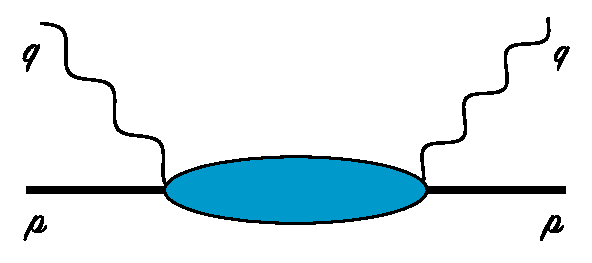
\includegraphics[width=5.5cm]{frwCSgeneric.eps}
\caption{Forward doubly-virtual Compton scattering: $N(p)+\gamma^*(q)\rightarrow N(p)+\gamma^*(q)$.  \label{fig:CSgeneric}}
\end{figure}

\section{The forward VVCS amplitude at N$\boldsymbol{^2}$LO} 
\label{Sec:ChEFT_for_VVCS}



\subsection{Lorentz decomposition and relation to structure functions} \seclab{LorentzDecomp}

Figure \ref{fig:CSgeneric} schematically shows the process of forward VVCS off the nucleon. 
The VVCS amplitude in forward kinematics can be decomposed in terms of four
independent Lorentz-covariant and gauge-invariant tensor structures
\cite{Hagelstein:2015egb}. Considering only the spin-independent part the amplitude has the form
%\begin{align}\label{Eq:T-Rel}
%T(\nu,Q^2) = \epsilon_{\mu}^{\prime *} \epsilon_\nu \Bigg\{  \Big( -g^{\mu \nu} + \frac{q^\mu q^\nu}{q^2} \Big) T_1(\nu,Q^2) + \frac{1}{M_N^2} \Big(  p^\mu - \frac{p\cdot q}{q^2} q^\mu \Big) \Big(  p^\nu - \frac{p\cdot q}{q^2} q^\nu \Big) T_2(\nu,Q^2) \nonumber \\ 
%                  +  \frac{i}{M_N} \epsilon^{\mu \nu \alpha \beta} q_\alpha s_\beta S_1(\nu,Q^2)   +\frac{i}{M_N^3} \epsilon^{\mu \nu \alpha \beta} q_\alpha (p\cdot q  s_\beta -s\cdot q  p_\beta ) S_2(\nu,Q^2)      \Bigg\}, 
%\end{align}
%where $s^\mu$ is the covariant spin tensor which satisfy $s\cdot p=0$ and $s^2=-1$, and the normalization of the Levi-Civita tensor is $\epsilon_{0123}=+1$. 
\bea
\label{Eq:T-Rel}
\hspace{-0.5cm}T(\nu,Q^2) & = &  \Bigg\{ 
\left( -g^{\mu\nu}+\frac{q^{\mu}q^{\nu}}{q^2}\right)
T_1(\nu, Q^2) +\frac{1}{M_N^2} \left(p^{\mu}-\frac{p\cdot
q}{q^2}\,q^{\mu}\right) \left(p^{\nu}-\frac{p\cdot
q}{q^2}\, q^{\nu} \right) T_2(\nu, Q^2)\eqlab{fVVCS}\Bigg\}\,\epsilon_{\mu}^{\prime *} \epsilon_\nu ,
\nn
\eea
with the incoming (outgoing) photon polarization vectors $\epsilon_\mu$ ($\epsilon_\mu^*$), the photon lab-frame energy $\nu$, the photon virtuality $Q^2=-q^2$ and the nucleon mass $M_N$.
The scalar functions $T_i$ parametrize the spin-independent part
of the amplitude. The relation of these functions to the conventional
laboratory-frame amplitudes can be found in Appendix
\ref{sec:SRVVCStensor}.

The optical theorem relates the absorptive parts of the forward VVCS amplitudes to the nucleon structure functions, or equivalently, to the cross sections of virtual photoabsorption:
\begin{subequations}
\eqlab{VVCSunitarity}
\bea
\im T_1(\nu,Q^2)&=&\frac{4\pi^2\al}{M_N}f_1(x,Q^2) \eqlab{ImT1}=K(\nu,Q^2)\,\sigma_T(\nu,Q^2), \\
\im T_2(\nu,Q^2)&=&\frac{4\pi^2\al}{\nu}f_2(x,Q^2)\eqlab{ImT2}=\frac{Q^2  K(\nu,Q^2) }{\nu^2+Q^2}\left[\sigma_T(\nu,Q^2)+\sigma_L(\nu,Q^2)\right], \\
\eea
\end{subequations}
with the fine structure constant $\alpha$ and the Bjorken variable $x=Q^2/2M_N \nu$. The photoabsorption cross sections, measured in electroproduction processes, are defined as $\sigma_T=\nicefrac12\, (\sigma_{1/2}+\sigma_{3/2})$, and $\sigma_L=\nicefrac12\, (\sigma_{1/2}+\sigma_{-1/2})$ for longitudinal photons, where the subscript on the right-hand side indicates the total helicity of the $\gamma^\ast N$ state. 
The flux of incoming particles in the photoabsorption process is described by the photon flux factor $K(\nu,Q^2)$. What is measured in experiment are not the photoabsorption cross sections $\sigma_i$ but actually $K \sigma_i$. Therefore, it is important to use the same flux factor in the derivation of the CS sum rules, entering through the optical theorem, and in the evaluation of the CS rum rules, entering by inserting the calculated cross sections. In our case, we use  Gilman's flux factor $K(\nu,Q^2)=|\vec{q}\,|=\sqrt{\nu^2+Q^2}$, where  $\vec{q}$ is the three-momentum of the photon in the laboratory frame. See Ref.~\cite{Drechsel:2002ar} for common flux factor choices, e.g., Hand's flux factor \cite{Hand:1963bb}.

The forward VVCS amplitudes satisfy dispersion relations derived from the general principles of analyticity and causality:
\begin{subequations}
\eqlab{genDRs}
\bea 
T_1 ( \nu, Q^2) &=&T_1(0,Q^2) + \frac{32\pi\al M_N\nu^2}{Q^4} \int_{0}^1 
\!\dd x 
\frac{x\, f_1 (x, Q^2)}{1 - x^2 (\nu/\nu_{B})^2 - i 0^+} \nonumber\\ 
&=& T_1(0,Q^2) + \frac{2\nu^2}{\pi } \int_{\nu_{B}}^\infty\! \frac{\dd \nu'}{\nu'} \, 
\frac{K(\nu',Q^2)\si_T ( \nu', Q^2)}{\nu^{\prime\,2} -\nu^2 - i 0^+}\,,\eqlab{T1dr}\\
T_2 ( \nu, Q^2) &=& \frac{16\pi\al M_N}{Q^2} \int_{0}^1 
\!\dd x\, 
\frac{f_2 (x, Q^2)}{1 - x^2 (\nu/\nu_{B})^2  - i 0^+} \nonumber \\
&=&\frac{2Q^2}{\pi} \int_{\nu_{B}}^\infty\! \dd \nu' \, 
\frac{\nu^{\prime}K(\nu',Q^2)[ \si_T+\si_L] ( \nu', Q^2)}{(\nu^{\prime\,2}+Q^2)(\nu^{\prime\,2} -\nu^2- i 0^+)} \eqlab{T2dr},\\
\eea 
\eqlab{SRgen}
\end{subequations}
with $\nu_{B}=Q^2/2M_N$ the elastic threshold. The unitarity relations given in \Eqref{VVCSunitarity}
thus connect the VVCS amplitudes to experimentally observable response functions. Note that the high-energy asymptotics of $f_1(x,Q^2)$ prevent the convergence of the corresponding unsubtracted dispersion integral,
giving rise to a once-subtracted dispersion relation, \Eqref{T1dr}, with the subtraction function $T_1(0,Q^2)$. 

A low-energy expansion (LEX) of \Eqref{genDRs} establishes various sum rules relating nucleon properties to experimental information on the photoabsorption cross sections \cite{Drechsel:2002ar,Hagelstein:2015egb}.
Low, Gell-Mann and Goldberger \cite{ Low:1954kd, Gell_Mann:1954kc} demonstrated that the leading terms in the LEX of the Compton scattering (CS) amplitudes are determined by the global properties of the nucleon: charge, mass and anomalous magnetic moment. These lowest-order terms represent the celebrated low-energy theorem (LET) \cite{Low:1954kd, Gell_Mann:1954kc}.
The polarizabilities, related to the internal structure of the nucleon,
enter the LEX as higher-order corrections. More details on the LEX of the VVCS amplitudes in terms of polarizabilities can be found in Appendix \ref{sec:SRVVCStensor}. 
An example of this is the well known Baldin sum rule~\cite{Baldin:1960}, that connects the sum of the electric and magnetic dipole polarizabilities
to the total photoabsorption cross section $\sigma_T$.
This sum rule can be generalized to the virtual-photon case~\cite{Drechsel:2002ar};
the virtual photon exchanged between the electron and the nucleon
in electron-nucleon scattering acts as a probe whose resolution depends on its virtuality $Q^2$.
In this way, one obtains information about the density of polarization inside the nucleon.
The definitions of the $Q^2$-dependent moments of structure functions considered in this paper are given in Section \ref{Sec:Scalar-Pol}.




 \begin{figure}[t]
 \centering
 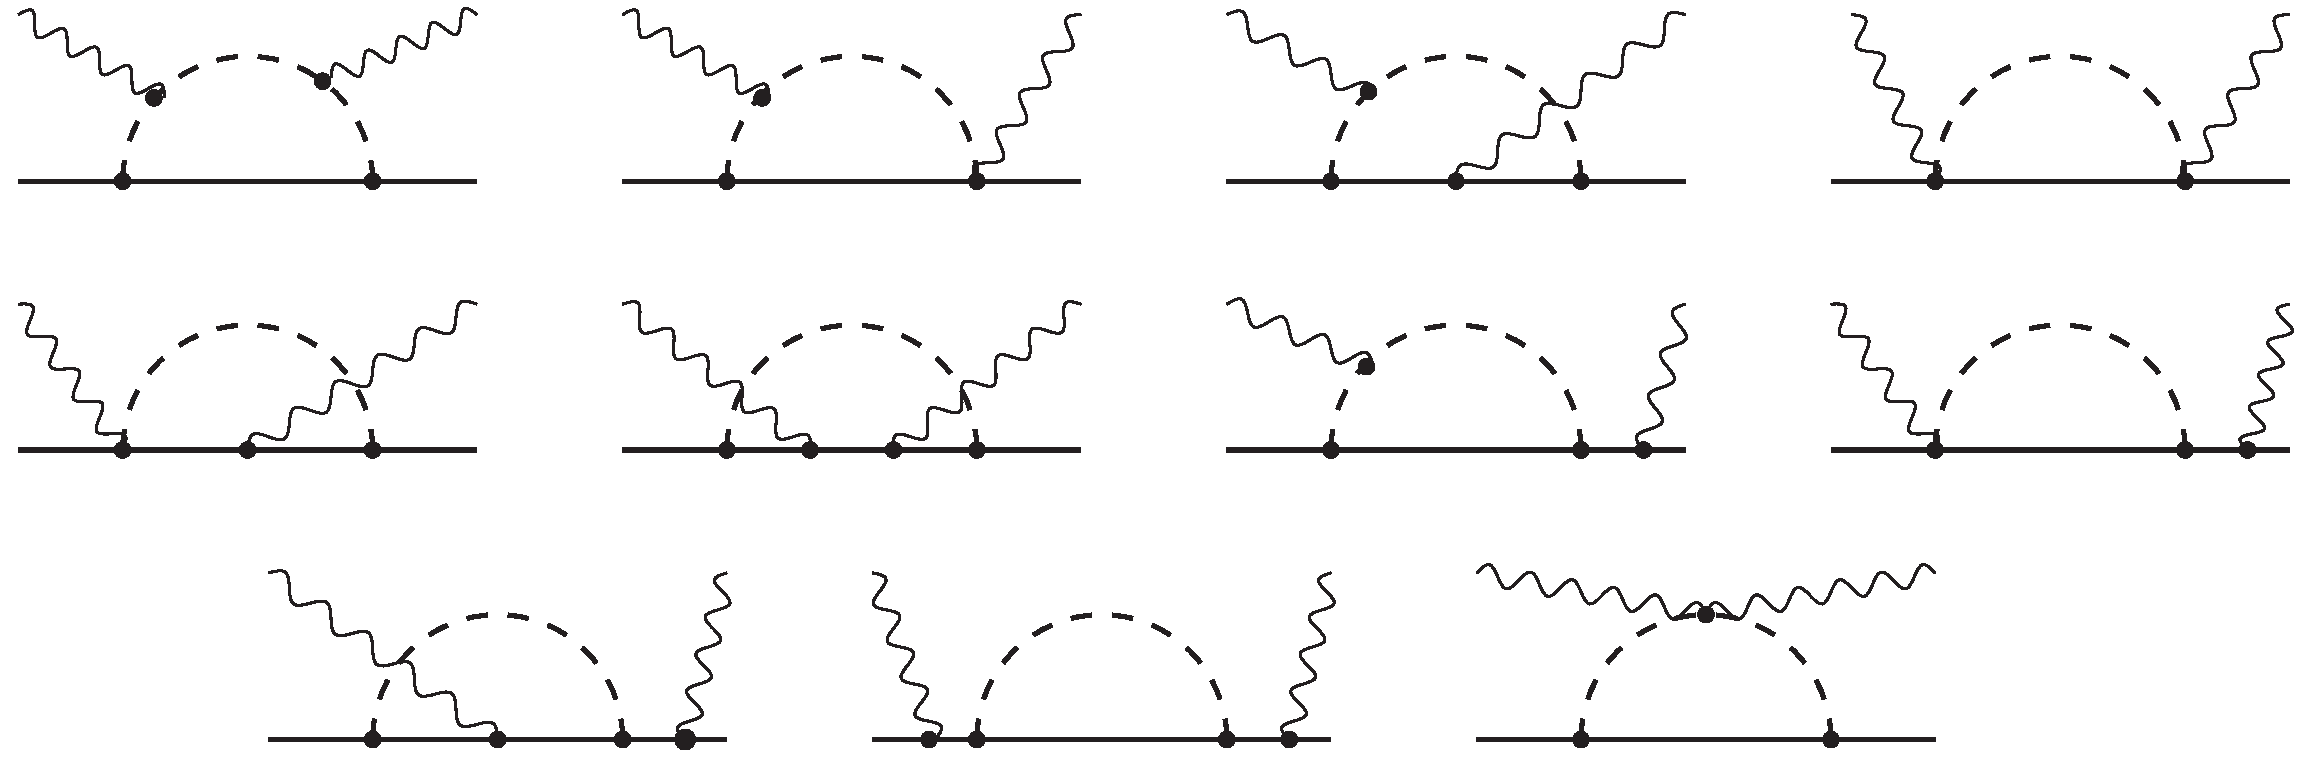
\includegraphics[width=0.95\columnwidth]{Diags1_pv.pdf} 
\caption{%(Color online)  
$\pi N$ one-loop graphs contributing to Compton scattering at $\mathcal{O}(p^3)$. Graphs obtained from these by
crossing and time-reversal are evaluated too.
}
\label{Fig:loops_pv}
\end{figure}



\begin{figure}
\centering
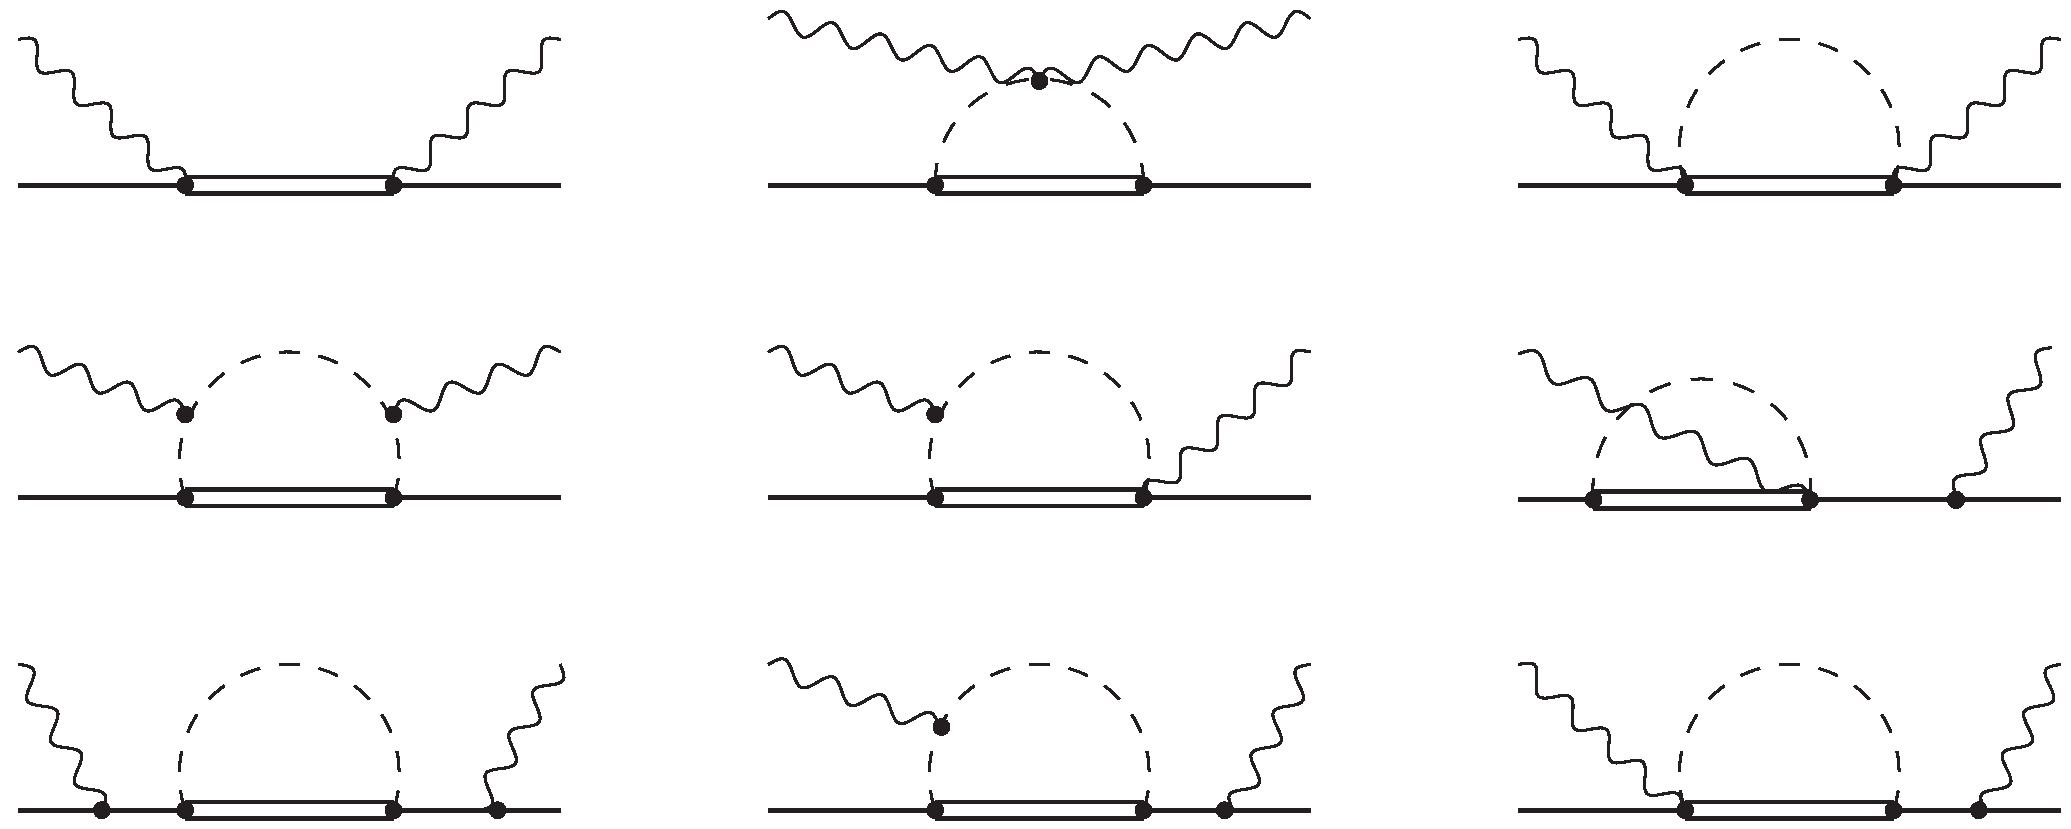
\includegraphics[width=0.9\columnwidth]{DeltaDiags4.pdf} 
\caption{%(Color online)  
Graphs contributing to Compton scattering at  $\mathcal{O}(p^4/\mathit{\Delta})$. 
Double lines denote the propagator of the $\Delta$ isobar.
Graphs obtained from these by
crossing and time-reversal are evaluated too.}
\label{Fig:loopsD}
\end{figure}

\subsection{Lagrangian and power counting}
We are computing the nucleon VVCS amplitudes $T_{1}$ and $T_{2}$
using SU(2) $\chi$PT \cite{Weinberg:1978kz,Gasser:1983yg},
including the nucleon and $\De(1232)$ 
degrees of freedom.  We shall employ B$\chi$PT, which is the manifestly-covariant extension of $\chi$PT to the single-baryon sector in its most straightforward
implementation, where
the nucleon
is included as in Ref.~\cite{Gasser:1987rb}\footnote{The power-counting concerns  
raised in Ref.~\cite{Gasser:1987rb} have been overcome by renormalizing away the ``power-counting
violation'' using the LECs (a.k.a., Wilson coefficients) available at that order.
 This has been shown explicitly within the  ``extended on-mass-shell renormalization scheme'' (EOMS)~\cite{Fuchs:2003qc}, 
 but is not limited to it.} and the $\De(1232)$ as in Ref.~\cite{Pascalutsa:2006up}. See also Ref.~\cite{Geng:2013xn} for a concise overview.
The heavy-baryon (HB) results can easily be obtained from B$\chi$PT by an additional expansion in the inverse powers of baryon masses. 




% We are working in the relativistic formulation of $\chi$PT with baryons
% including the $\Delta(1232)$-resonance as a dynamical degree of freedom.
% This calculation generalizes the work of Ref.~\cite{Lensky:2009uv} to the case of virtual photons in the forward kinematics.
% The potential of the covariant formalism, once the $\Delta(1232)$ is included as an explicit degree of freedom,
% has also been observed in other chiral analyses of, e.g., $\pi N$ scattering~\cite{Alarcon:2012kn,Chen:2012nx}
% and $\pi N \to \pi \pi N$ \cite{Siemens:2014pma}. 

% We employ the chiral Lagrangian for the pion and nucleon fields, see Ref.~\cite{Gasser:1987rb}. Up to second order in the pion field, it takes the form:
% \bea
% \mathcal{L}^{(1)}_{N}  &=&  \overline{N}\left( i \slashed{\partial} -{M}_{N}
% + \frac{g_A}{2f_\pi} \tau^a \slashed{\partial}\,\pi^a\gamma_5\right.\\
% &&\left.- \frac{1}{4f_\pi^2} \, \tau^a \epsilon^{abc}  \pi^b\,\slashed{\partial} \,\pi^c
% \right) N  + \mathcal{O}(\pi^3) \,,
% \label{expNlagran}\nn
% \eea
% where $g_A$ is the nucleon axial coupling, $f_\pi$ is the pion weak decay constant and $\tau^a$ are the Pauli matrices.
% The Lagrangian of the $\Delta(1232)$-isobar field and its coupling to the nucleons and pions is~\cite{Pascalutsa:2003aa,Lensky:2009uv}:
% \bea
% \mathcal{L}^{(1)}_{\Delta} &=& \overline\Delta_\mu \left(i\gamma^{\mu\nu\lambda}\,\partial_\lambda - 
% M_\Delta\,\gamma^{\mu\nu}\right) \Delta_\nu  \\
% &&-\frac{h_A}{2f_\pi M_\Delta}
% \left[ \overline N\, T_a%^\dagger
%  \,\gamma^{\mu\nu\lambda}\, (\partial_\mu \Delta_\nu)\, \partial_\lambda\pi^a
% + \mbox{H.c.}\right],\nn
% \eea
% where $M_\Delta$ is the mass of the $\Delta(1232)$, $h_A$ is the $\pi N\Delta$ coupling and $T^a$ are the isospin $1/2\rightarrow 3/2$ transition matrices.
% The electromagnetic interaction is added via the minimal substitution:
% \begin{subequations}
% \bea
% \partial_\mu N &\to&  \partial_\mu N -  i e A_\mu\frac{1}{2}(1+\tau_3) N ,\\
% \partial_\mu \pi^a &\to&  \partial_\mu \pi^a - eA_\mu\epsilon^{ab3}\pi^b\,,
% \eea
% \end{subequations}
% where $A_\mu$ is the photon field and $e=\sqrt{4\pi \al}$. The minimal coupling of the photon to the delta field gives contributions to Compton scattering (CS) which are of higher orders than the ones considered in this work. 

Let us recall that  chiral effective-field theory is based on 
a perturbative expansion in powers of pion momentum $p$ and mass $m_\pi$ over the scale of spontaneous chiral symmetry breaking ${\Lambda_\chi\sim 4\pi f_\pi}$, with
$f_\pi\simeq 92$~MeV the pion decay constant. Each operator in the effective Lagrangian, or a
graph in the loopwise expansion of the S-matrix, can have a specific order of
$p$ assigned to it.
To give a relevant example consider the following operator: 
\beq
\bar N N F^2,
\eeq
with $N$ standing for the Dirac field
of the nucleon, and $F^2$ the square of the electromagnetic field strength tensor, $F_{\mu\nu}=\pa_{[\mu}A_{\nu]}$. This is an operator of $\mathcal{O}(p^4)$. Two of the $p$'s come from the
photon momenta which are supposed to be small, and the other two powers arise because the two-photon
coupling to the nucleon must carry a factor of $\al$ (the charge $e$ counts as $p$, since we want
the derivative of the pion field to count as $p$ even after including the minimal coupling to the photon).

This operator enters the effective Lagrangian with a LEC, denoted by $C$,
and it gives a contribution to the CS amplitude in the form of\footnote{
Throughout this paper we use the conventions summarized in the beginning of Ref.~\cite{Hagelstein:2015egb}.}
\beq 
\mathcal{M}^{\mu\nu}_C = C \, (q\cdot q' \, g^{\mu\nu} - q^\mu q^{\prime\,\nu}).
\eeq 
Hence, it leads to a shift in the magnetic dipole polarizability: $\be_{M1}\to \be_{M1}+C/4\pi$.
Now, two important remarks are in order.
\begin{itemize}
\item[i)] {\em Naturalness}. The value of $C$ is not completely arbitrary, but rather goes as 
${C= (e^2/\La_\chi^3) c} $, with the dimensionless constant $c$ being of the order of 1, or more precisely:
\beq 
p/\La_\chi \ll |c|\ll \La_\chi/p\,.
\eeq 
This condition ensures that the contribution  of this operator is indeed 
of $\mathcal{O}(p^4)$, as the power counting commands.
\item[ii)] {\em Predictive powers}.
This LEC enters very prominently in the polarizabilities and CS  at tree level,
which means its value is best fixed by the empirical information on these quantities. 
If this is so, the $\mathcal{O}(p^4)$ result is not ``predictive'', as it could only be used to {\em fit} 
the $\chi$PT expression to experiment or lattice QCD calculations. On the other hand, contributions
of orders lower than $p^4$ are predictive, as they only contain LECs fixed from elsewhere.
It is crucial to first study the predictive contributions, if there are any, and this is what we shall
focus on here.
\end{itemize}

The ``predictive'' contributions to CS and polarizabilities have been identified  and computed  for the case
of RCS \cite{Lensky:2009uv}, 
VCS \cite{Lensky:2016nui}, and  VVCS \cite{Lensky:2014dda}.
Our present calculation is quite analogous to those works and hence 
we refer to them for most of the technical details, such as the expressions for the
relevant terms of the effective Lagrangian. We have to note, however,
that we include the Coulomb-quadrupole $(C2)$ $N\to \Delta$ transition,
described by the $g_C$ term in the following non-minimal $\gamma^* N \Delta$ coupling~\cite{Pascalutsa:2005vq,Pascalutsa:2005ts}:\footnote{Note that Refs.~\cite{Pascalutsa:2005ts,Pascalutsa:2005vq,Pascalutsa:2006up} have the wrong sign for the $g_C$ term.}
\bea
\mathcal{L}^{(2)}_\Delta &=&  \frac{3e}{2M_N M_+}\,\overline N\, T_3\,\Big\{
i g_M  \tilde F^{\mu\nu} \,\partial_{\mu}\Delta_\nu- g_E \gamma_5 F^{\mu\nu}\,\partial_{\mu}\Delta_\nu\eqlab{gammaNDeltaLag}\\
&& +i \frac{g_C}{M_\Delta}\gamma_5 \gamma^\alpha (\partial_\alpha \Delta_\nu-\partial_\nu \Delta_\alpha)\partial_\mu F^{\mu \nu}\Big\}+\,\mbox{H.c.},
\nn
\eea
with $M_+=M_N+M_\Delta$ and the dual of the electromagnetic field strength tensor
%and $F^{\mu\nu}$ and $\tilde F^{\mu\nu}$ are the conventional electromagnetic field strength tensor and its dual, $F^{\mu\nu}=\partial^\mu A^\nu-\partial^\nu A^\mu$ 
 $\tilde F^{\mu\nu}=\frac{1}{2}\epsilon^{\mu\nu\rho\lambda}F_{\rho\lambda}$.
The electric, magnetic and Coulomb couplings ($g_E$, $g_M$ and $g_C$)
are known from the analysis of pion photoproduction $P_{33}$ multipoles~\cite{Pascalutsa:2005ts}.
The corresponding numerical values, as well as those of other physical constants used in this work, are given in Table~\ref{tab:constants}. The Coulomb coupling is subleading
compared with the electric and magnetic couplings, and it was not included in the previous calculations.
However, the relatively large magnitude of $g_C$ hints at its potential numerical importance,
which we examine in this work.

\begin{table}[b]
\caption{Parameters (fundamental and low-energy constants) \cite{Agashe:2014kda} at the order they appear first. The $\pi N\Delta$ coupling constant $h_A$ is fit to the experimental Delta width and the $\gamma^* N \Delta$ coupling constants $g_M$, $g_E$ and $g_C$ are taken from the pion photoproduction study of Ref.~\cite{Pascalutsa:2005vq}.\label{tab:constants}} 
\begin{tabular}{lp{0.3cm}l}
\hline
$\mathcal{O}(p^2)$&&$\alpha=1/(137.04)$, $M_N=M_p=938.27$ MeV\\
$\mathcal{O}(p^3)$&&$g_A=1.270$, $f_\pi=92.21$ MeV, $m_\pi=139.57$ MeV \\
$\mathcal{O}(p^4/\varDelta)$&&$M_\Delta=1232$ MeV, $h_A\equiv 2g_{\pi N \Delta}=2.85$, $g_M=2.97$, $g_E=-1.0$, $g_C=-2.6$\\
\hline
\end{tabular}
\end{table}

On the conceptual side, it is important to note that the counting of the $\De(1232)$ effects is done in the so-called ``$\delta$-counting''~\cite{Pascalutsa:2003aa}. In it, the Delta-nucleon mass difference,
$\varDelta=M_\Delta-M$, is counted as a light scale ($\varDelta \ll \La_\chi$) which is
substantially heavier than the pion mass ($m_\pi\ll\varDelta)$. Hence, if $p\sim m_\pi$, 
then $\mathcal{O}(p^4/\varDelta)$ is in between of $\mathcal{O}(p^3)$ and $\mathcal{O}(p^4)$. 


For the non-Born VVCS amplitudes
and polarizabilities the predictive orders are $\mathcal{O}(p^3)$ and $\mathcal{O}(p^4/\varDelta)$.
The $\mathcal{O}(p^3)$ contribution comes from the pion-nucleon ($\pi N$) loops shown in Fig.~\ref{Fig:loops_pv}.
We refer to it here as the leading-order (LO) contribution.\footnote{In the full Compton amplitude (i.e., 
including the Born term) it is, in fact, a next-to-leading-order contribution, and this is how it is referred to sometimes, e.g.~in Ref.~\cite{Lensky:2009uv}. }
The $\mathcal{O}(p^4/\varDelta)$ contribution, arising at the NLO, 
comes from the Delta-exchange ($\Delta$-exchange) graph and the pion-Delta ($\pi \Delta$) loops shown in Fig.~\ref{Fig:loopsD}.

The $\Delta$-exchange graph in Fig.~\ref{Fig:loopsD} is described by the $\gamma^* N \Delta$ interaction in \Eqref{gammaNDeltaLag}. For the magnetic coupling, one assumes a dipole behavior to mimic the form expected from 
vector-meson dominance:
\begin{equation}
g_M\to \frac{g_M}{\big[1+\left(Q/\Lambda\right)^2\big]^2}\,,
\end{equation}
with the dipole mass $\Lambda^2=0.71$~GeV${^2}$. The inclusion of this $Q^2$ dependence is motivated by observing the importance of this form factor for the correct description of the electroproduction data \cite{Pascalutsa:2005vq}. Since electroproduction off the nucleon is directly connected with the nucleon polarizabilities via sum rules, it is understandable that a better description of the electroproduction data will lead to a better description of the $Q^2$ behavior of the polarizabilities. The effect of the dipole form factor in $g_M$ is illustrated in Fig.~\ref{Fig:alpha+beta-orders}.

% In what follows, a N$^2$LO B$\chi$PT calculation of
% the nucleon VVCS amplitudes is presented.  In particular, we are studying the non-Born part, i.e., everything but the leading-order (LO) Born diagrams of elastic tree-level CS. The Born amplitudes are completely described by elastic form factors, whereas the non-Born amplitudes are related to polarizabilities. Therefore, our calculation of
% the nucleon VVCS amplitudes at N$^2$LO in B$\chi$PT gives the nucleon polarizabilities at NLO. At this order in the $\delta$-counting, the chiral approach is free of unknown LECs, thus, 
% provides predictions of the polarisabilities.


% The Feynman diagrams evaluated by us are shown in Figs.~\ref{Fig:loops_pv} (NLO) and \ref{Fig:loopsD} (N$^2$LO).\footnote{Note that a chiral rotation of the nucleon field can considerably simplify the calculation of the $\pi N$ one-loop diagrams~\cite{Lensky:2009uv}.}
%  In analogy with Ref.~\cite{Pascalutsa:2005vq}, we take into account the effect of the $\gamma^* N \Delta$ transition form factor
% (entering the corresponding vertex in the $\Delta$-exchange graph in Fig.~\ref{Fig:loopsD}) by introducing the following running
% of the magnetic $\gamma^* N \Delta$ coupling:
% \begin{align}
% g_M \to \frac{g_M}{(1+ Q^2/\Lambda^2 )^2 },\eqlab{dipolegm}
% \end{align} 
% where $\Lambda=\sqrt{0.71~\text{GeV}^2}\approx 0.84$~GeV. 
% The inclusion of this $Q^2$ dependence is motivated by previous works which point out the importance of this form factor in the correct reproduction of the electroproduction data \cite{Pascalutsa:2005vq}. 

A feature of the $\delta$-counting is that the characteristic momentum
$p$ distinguishes two regimes: the {\it low-energy} ($p\simeq m_\pi$) and 
{\it resonance} ($p\simeq \varDelta$) regimes. The above counting is limited to the 
low-energy regime.
Since we are interested in the LEX of the  VVCS amplitudes (i.e., $\nu=0$ with $Q^2$ finite),
we do not consider the regime where one-Delta-reducible graphs are enhanced (resonance regime).
However, going to higher $Q^2$ one does need to count the 
Delta propagators similar to the nucleon propagators, which, in turn, calls for inclusion
of $\pi \Delta$ loops with two and three Delta propagators, which have been omitted here. They are only included implicitly 
 by adjusting the isospin coefficients of the one-nucleon-reducible graphs in Fig.~\ref{Fig:loopsD} to restore current conservation, as explained in the next section. Apart from that, $\pi \Delta$ loops have a rather mild
dependence on momenta and the missing loops are unlikely to  affect the
$Q^2$-dependence of the moments of structure functions significantly, even for $Q^2$ comparable to $\varDelta^2$. 





Note also that the $\pi^0$ anomaly graph, which enters the VVCS amplitude at $\mathcal{O}(p^2)$
and is sometimes considered together with the Born term, does not contribute to the considered moments.



% Our approach to evaluate the loop diagrams in Figs.~\ref{Fig:loops_pv} and \ref{Fig:loopsD} closely follows the one of Ref.~\cite{Lensky:2009uv},
% with the necessary modifications due to the different kinematical regime. In particular, the gauge condition used in Refs.~\cite{Pascalutsa:2003aa,Lensky:2009uv}
% is dropped, and the terms relevant for the virtual photon case are restored everywhere in the loop integrals.
% The latter are first written in the Feynman parameterisation, and the covariant amplitudes $T_{1,2}(\nu,Q^2)$, $S_{1,2}(\nu,Q^2)$
% are obtained by matching the corresponding tensor structures in Eq.~(\ref{Eq:T-Rel}).\footnote{It is interesting to note that the tensor decomposition provides a non-trivial test of the calculation: we encountered additional tensor structures
% that violated the gauge invariance; however, the scalar integrals over the Feynman parameters that multiplied these non-gauge-invariant structures
% vanished after evaluation.}

\subsection{Renormalization}

The calculation of the $\pi N$- and $\pi\Delta$-loop graphs in Figs.~\ref{Fig:loops_pv} and \ref{Fig:loopsD} is analogous to Ref.~\cite{Lensky:2009uv}, with the obvious extension to the case of a finite photon virtuality. The renormalization is also done in the exact same way; 
namely, graphs with the nucleon self-energy
or  one-loop $\gamma NN$ vertices are subtracted according to
the usual prescription:
\begin{align}
\Sigma_R(\slashed{p}_s)&=\Sigma(\slashed{p}_s)-\Sigma(\slashed{p})-\Sigma'(\slashed{p})(\slashed{p}_s-M)\,,\eqlab{selfenergy}\\
\Gamma^\mu_R(p,p')&=\Gamma^\mu(p,p')-\Big[\gamma^\mu F_1(q^2)
-\frac{1}{2M}\gamma^{\mu\nu}q_\nu F_2(q^2)
\Big]\,,\eqlab{oneloopvertex}
\end{align}
where $p_s$ and $p$ in \Eqref{selfenergy} are the off-shell and the on-shell momentum of the nucleon, and
$F_1(q^2)$ and $F_2(q^2)$ in \Eqref{oneloopvertex} are the on-shell nucleon Dirac and Pauli form factors
resulting from the unsubtracted $\gamma NN$ vertex $\Gamma^\mu(p,p')$, with $q=p'-p$
being the momentum transfer from the photon to the nucleon.
Note that this procedure corresponds
to subtracting the Born contribution from the VVCS process.
The $\pi \Delta$-loop graphs
still contain divergences after this subtraction. These divergences are of higher orders, $\mathcal{O}(p^5/\varDelta^2)$ and  $\mathcal{O}(p^4)$,
and will be cancelled by the corresponding higher-order
contact terms. In practice, they are removed by taking the $\overline{\text{MS}}$ values of the divergent quantities.

As mentioned above, $\pi \Delta$-loop graphs where photons couple minimally to the Delta contain more 
than one Delta propagator and therefore should be suppressed by extra powers of $p/\varDelta$.
However, their lower-order contributions are important for electromagnetic gauge invariance and therefore for the 
renormalization procedure. In particular, the lower-order contributions of chiral loops should not affect the result of the LET~\cite{ Low:1954kd, Gell_Mann:1954kc}, and this condition is automatically satisfied by a subset of graphs if it obeys gauge invariance. The loop graphs in 
Fig.~\ref{Fig:loopsD} form such a subset for the case of the neutral Delta. In reality, the Delta comes in four charge states (isospin $3/2$), thus, a 
gauge-invariant set will in addition have the higher-order graphs where the photon couples minimally to the Delta. To make the subset of loop graphs 
in Fig.~\ref{Fig:loopsD} gauge invariant without the higher-order graphs, we used the same procedure as in Ref.~\cite{Lensky:2009uv}. The one-particle-irreducible (1PI) graphs in Fig.~\ref{Fig:loopsD} are computed with the correct isospin factors, i.e., summing over all charge 
states of the Delta, whereas the isospin factors for the one-particle-reducible (1PR) loop graphs are chosen such that their ratio to the isospin factors
of 1PI graphs is the same as in the neutral Delta case. This procedure automatically ensures exact gauge invariance and thus 
effectively includes the relevant contributions of the one-loop graphs with minimal coupling of photons to the Delta. If the latter graphs 
are included explicitly, the isospin factors of 1PR graphs can be restored to actual values.
The corresponding change in the values of the polarizabilities, however, is of higher order than what we consider in this work.



% The renormalization proceeds in the same way as described in Ref.~\cite{Lensky:2009uv}, with one important modification: as argued in
% Ref.~\cite{Birse:2012eb} (see also Ref.~\cite{Alarcon:2013cba}), we subtract from the $\gamma^* NN$-loop graphs, which enter the 1PR graphs,
% the structures that correspond to the on-shell elastic nucleon vertex rather than just renormalize the nucleon charge and anomalous magnetic moment.
% \textcolor{red}{This means that in the loop $\gamma^* NN$ vertex function,}
% \bea
% \Gamma^\mu(\nu,Q^2)&=&F_1(\nu,Q^2)\gamma^\mu+F_2(\nu,Q^2)\gamma^{\mu\rho}q_\rho\\
% &&+F_3(\nu,Q^2)p^\mu\slashed{q}+F_4(\nu,Q^2)(\slashed{p}+\slashed{q}-M_N)\gamma^\mu\,,\nn
% \eea

\subsection{Uncertainty estimate}
%In making comparison with experimental data, it is important to provide a theoretical uncertainty. In the case of an EFT expansion, the common way to obtain this uncertainty is via the estimate of higher-order contributions. This work employs the following estimate. In the low-momenta regime, where the expansion parameter is $\displaystyle\delta\sim p/\varDelta$, our calculation is of the next-to-leading order (NLO). A conservative estimate of the next-to-next-to-leading order (NNLO) contributions would be $\text{error}(f)=\delta^2 f$, where $f$ is a generic VVCS amplitude or response function. It is important to note, however, that the error of the scalar polarizabilities $\alpha_{E1}(Q^2)$ and $\beta_{M1}(Q^2)$ in the static limit $Q^2=0$ is defined by the error of the corresponding static (real) polarizabilities. This error was argued to be small~\cite{Lensky:2015awa} due to the fact that these polarizabilities are very close at NLO to the results obtained in B$\chi$PT fits to real Compton scattering data~\cite{Lensky:2014efa}, and that there are contact terms at NNLO that will in any case compensate changes in $\alpha_{E1}$ and $\beta_{M1}$ coming from other higher-order mechanisms. The static errors are estimated  as $\text{error}(\alpha_{E1},\text{static})\simeq\text{error}(\beta_{M1},\text{static})\sim 0.7\times 10^{-4}$~fm${^3}$ (see Ref.~\cite{Lensky:2015awa}); this translates to the uncertainty of $4.7$~GeV${^2}$ and $2.3$~GeV${^2}$ in $P_{LL}(0)$ and $P_{LT}(0)$, respectively. This static uncertainty has to dominate at very small $Q^2$, whereas at larger $Q^2$ (still in the low-momenta regime) the term $\delta^2 f\sim (p^2/\varDelta^2) f$ will become more important. In practice, we take the sum of the two values.

%The uncertainty estimate in the high-momenta regime works in a similar way. In this regime, $p\gtrsim\varDelta$, our calculation is at an incomplete leading order (LO), however, we will treat it as an LO calculation as argued above. The expansion parameter in this regime can be one of these, \beq\nonumber 
%\delta
%=\left\{\frac{m_\pi}{\varDelta},\frac{p}{\Lambda_\chi},\frac{\varDelta}{\Lambda_\chi}\right\}\,,
%\eeq
%and we take the average value of the three in order to estimate the NLO contribution. In summary, our uncertainty estimate for a VCS amplitude or a response function $f$ is given by
%\begin{equation}
%\text{error}(f)=
%\left\{
%\begin{matrix}
%%\Delta^\mathrm{st}
%\text{error}(f,\text{static})+\displaystyle\frac{p^2}{\varDelta^2}f\,, & p\lesssim \varDelta\,,  \\
%& \\
%\displaystyle\frac{1}{3}\left(\frac{m_\pi}{\varDelta}+\frac{p}{\Lambda_\chi}+\frac{\varDelta}{\Lambda_\chi}\right)f\,, & p\gtrsim\varDelta\,,
%\end{matrix}
%\right.
%\end{equation}
%where $\text{error}(f,\text{static})$
%is the static uncertainty discussed above. To obtain
%smooth bands in the plots, the uncertainties in the different regimes
%are multiplied by smooth transition functions. 

%\textcolor{red}{One has to note that this error estimate can lead to artefacts such as zero crossings, in the regime $p\gtrsim\varDelta$: the error being proportional to the observable, it can become small or even turn to zero if the latter decreases or vanishes. While we still consider this issue to be tolerable as far as the plots we demonstrate here are concerned, one can see it manifest, for instance, in Figs.~\ref{fig:response_function_PLT} and~\ref{fig:alpha_beta} below, where the bands of $P_{LT}$ and $\beta_{M1}$ shrink at larger values of $Q^2$. {\color{blue} Remove the zero crossing discussion or adjust it to the text --- mention $I_A$ and $\bar{d}_2$ as examples?}}




To estimate the uncertainties of our NLO predictions, we define
\begin{align}
 \tilde{\delta}(Q^2) = \sqrt{ \left(\frac{\varDelta}{M_N}\right)^2 + \left(\frac{Q^2}{2 M_N \varDelta}\right)^2 },\eqlab{dtilde}
\end{align}
such that the next-to-next-to-leading order (N$^2$LO) is expected to be of relative size $\tilde{\delta}^2$ \cite{Pascalutsa:2005vq}.

The slope of $\al_{E1}+\be_{M1}$ at the real-photon point turns out to be very small. Its smallness  suggests a cancellation of leading orders, thus, we estimate their relative error as $\tilde{\delta}$. 

%Since  the individual contributions from $\pi N$ loops, $\Delta$ exchange and $\pi \Delta$ loops  to $\gamma_0^p$, $\gamma_0^n$ and $I_A^p$ cancel each other for certain values of $Q^2$, we estimate the error of these polarizabilities as their largest (absolute) value in the $Q^2$ domain considered multiplied by $\tilde \delta$.

%We should also note that the zero values of $I_A(0)$, $I_1(0)$ and $\Gamma_1(0)$ are given by the elastic Pauli form factor, which is not part of our B$\chi$PT calculation and is considered to be exact.
%{\color{blue} Here, we have to describe the new error estimate!}

% Note that the procedure, described above, to make the $\pi \Delta$ loop graphs subset gauge invariant,
% also makes them give the same contributions for the neutron and for the proton. On the other hand, the $\pi N$ loop contribution
% to the neutron polarizabilities can be calculated from tree level pion electroproduction graphs as described below,





\section{Results and discussion}

In this section, we present the B$\chi$PT predictions for the nucleon polarizabilities and some moments of the nucleon structure functions, obtained from the LEX of the VVCS amplitudes. In addition to providing the full NLO results, we also analyse the individual contributions from the $\pi N$ loops, the $\Delta$ exchange, and the $\pi \Delta$ loops.

%\section{Scalar Polarizabilities}
\label{Sec:Scalar-Pol}

\subsection{Electric and magnetic dipole polarizabilities}


\begin{figure}[hbt]
\begin{center}
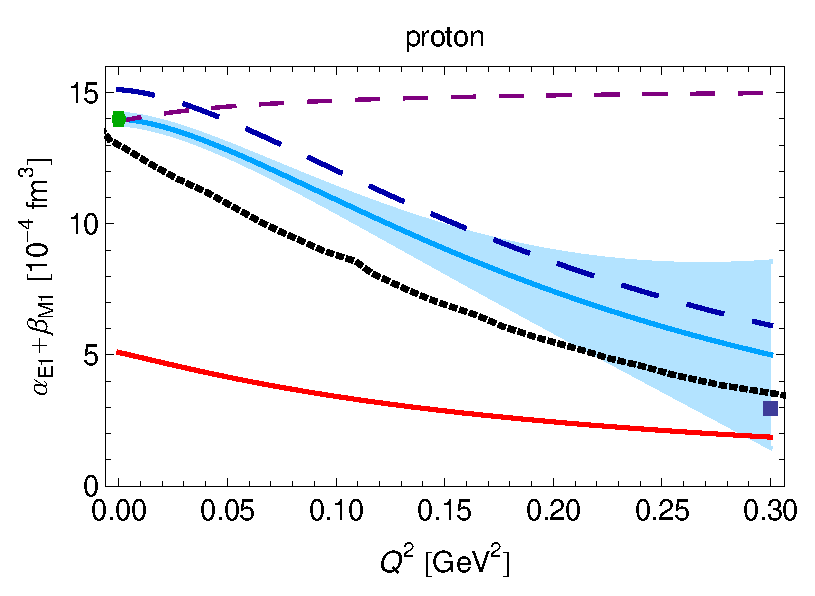
\epsfig{file=alpha+beta_p-Dip.eps,width=6.5cm,angle=0} \hspace{0.5cm}
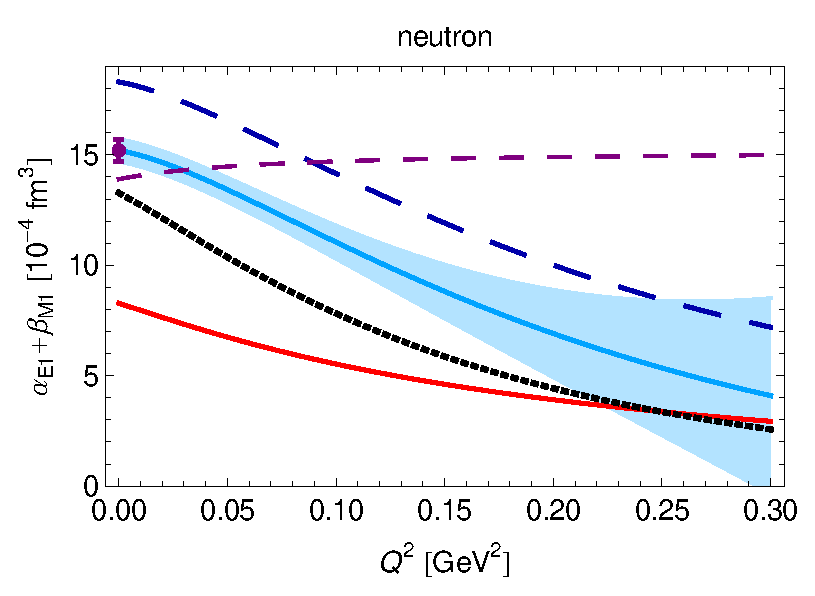
\epsfig{file=alpha+beta_n-Dip.eps,width=6.5cm,angle=0} 
\caption{Sum of electric and magnetic dipole polarizabilities, $\alpha_{E1}(Q^2)+\beta_{M1}(Q^2)$, for the proton ($p$) and neutron ($n$) as function of $Q^2$.  
The result of this work is shown by the blue solid line and the blue band.
The red line represents the LO B$\chi$PT result, while the blue dashed line is the LO HB limit~\cite{Nevado:2007dd}.
The black dotted line is the MAID model prediction~\cite{Drechsel:2000ct,Drechsel:1998hk,private-Lothar}; note that for the proton we use the updated estimate from Ref.~\cite{Drechsel:2002ar} obtained using the $\pi+\eta+\pi\pi$ channels.
At $Q^2=0$~GeV$^2$, we show Baldin sum rule evaluations for the proton (green dot)~\cite{Gryniuk:2015aa} and neutron (purple dot)~\cite{Babusci:1997ij}.
 The $Q^2=0.3$~GeV$^2$ point (blue dot) is an evaluation of the generalized Baldin sum rule \cite{Liang:2004tk}.
 \label{Fig:alpha+betaplot}}
\end{center}
\end{figure}


The electric and magnetic dipole polarizabilities, $\alpha_{E1}(Q^2)$ and $\beta_{M1}(Q^2)$, encode information about the dipole response of the nucleon to an electromagnetic field. For finite momentum transfers, the sum of the dipole polarizabilities is given by the generalized Baldin sum rule:
\beq
[\alpha_{E1}+\beta_{M1}] (Q^2)= \frac{1}{2 \pi^2} \int_{\nu_0}^\infty \! \dd\nu'\,\frac{K(\nu',Q^2)}{\nu'} \frac{\sigma_T (\nu',Q^2)}{\nu'^2} =\frac{8 \al M_N}{Q^4}\int_0^{x_0}\!\dd x\, x \,f_1(x,Q^2),\label{Eq:alpha+betaQ2}
\eeq
where $\nu_0$ is the lowest inelastic threshold, in this case the one-pion production threshold $\nu_0=m_\pi + (m_\pi^2+Q^2)/2M_N$, and $x_0=Q^2/2M_N \nu_0$.
%The information encoded in these polarizabilities is of major interest to extract the proton radius from the measurement of the $\mu$H Lamb shift \cite{Birse:2012eb,Alarcon:2013cba,Carlson:2011zd,Nevado:2007dd,Peset:2014yha,Hagelstein:2017cbl}, since they provide the structure corrections needed for an accurate extraction of the proton radius.
The electric and magnetic dipole polarizabilities of the nucleon enter the nucleon-structure contributions
to the Lamb shift of $\mu$H and other muonic atoms \cite{Bernabeu:1982qy,Pachucki:1996zza,Carlson:2011zd,Alarcon:2013cba}, and thus
are of major interest for an accurate extraction of the nuclear charge radii.

Our B$\chi$PT predictions for $\alpha_{E1}+\beta_{M1}$ are shown in Fig.~\ref{Fig:alpha+betaplot}, both for the proton
and the neutron, up to photon virtualities of $0.3$~GeV$^2$. We show our complete NLO results, which include the $\pi N$-loop, the $\Delta$-exchange and the $\pi \Delta$-loop contributions. In order to illustrate the effect of the Delta in these predictions, we also plot the LO $\pi N$-loop contribution
separately. We compare our results for the $Q^2$
evolution with the LO HB$\chi$PT predictions~\cite{Nevado:2007dd} and the MAID model predictions~\cite{Drechsel:2000ct,Drechsel:1998hk}. The latter are based on the generalized Baldin sum rule~\eqref{Eq:alpha+betaQ2} evaluated with ($\pi+\eta+\pi \pi$) photoproduction
cross sections~\cite{Drechsel:2002ar}. 
The data point are also evaluations of the (generalized) Baldin sum rule \cite{Liang:2004tk,Gryniuk:2015aa,Babusci:1997ij}. One can see that the B$\chi$PT predictions seem to systematically overestimate the MAID model in the $Q^2$ range shown here. 

The LO HB results seem to agree with the empirical values at the real-photon point~\cite{Babusci:1997ij}
both for the proton and the neutron. However, they do not fall off with increasing $Q^2$ in contrast to the B$\chi$PT predictions.
This asymptotic behavior is the reason for the large proton-polarizability effect on the muonic-hydrogen Lamb shift found within HB$\chi$PT \cite{Nevado:2007dd,Peset:2014yha}, much larger than the phenomenological value. As shown in Ref.~\cite{Alarcon:2013cba,Lensky:2017bwi}, this issue is solved within the relativistic formulation, which gives a result closer to calculations based on the dispersive approach.


The RCS dipole polarizabilities $\alpha_{E1}$ and $\beta_{M1}$ have been separately studied both within the HB  and
the covariant $\chi$PT. While  HB$\chi$PT gives results
remarkably close to the experimental determinations already at LO \cite{Bernard:1995dp},
the contribution of the $\Delta(1232)$ is harder to accommodate in this framework~\cite{Hemmert:1996rw}. In contrast to that, LO  B$\chi$PT \cite{Bernard:1991rq,Bernard:1991ru}
yields smaller values for the sum of dipole polarizabilities, in disagreement with the empirically extracted values based on evaluations of the Baldin sum rule with modern photoabsorption data~\cite{Babusci:1997ij,Olm01,Gryniuk:2015aa}. However, the NLO contributions from $\Delta$ exchange and $\pi\Delta$ loops improve the situation \cite{Lensky:2009uv,Lensky:2015awa}.
In the case of the proton, they bring the B$\chi$PT result in agreement with the experimental extraction, while for the neutron the total result is slightly bigger. The $\Delta(1232)$ contributions are therefore naturally accommodated in  B$\chi$PT but not in HB$\chi$PT.
%{\color{blue} We may need to give newer references here.}

The B$\chi$PT contributions from $\pi N$ loops, $\Delta$ exchange and $\pi \Delta$ loops to the static polarizabilities are, in that order and in the usual units of $10^{-4}$~fm$^3$:
\begin{align}
\alpha_{E1}^p+\beta_{M1}^p=15.12(1.48) \approx 5.10+7.04+2.98, \label{Eq:alpha+betaProtonRealPoint}\\
\alpha_{E1}^n+\beta_{M1}^n =18.30(1.79)\approx 8.28+7.04+2.98. \label{Eq:alpha+betaNeutronRealPoint}
\end{align}
The corresponding individual contributions to the $Q^2$-dependent generalized polarizabilities are shown in Fig.~\ref{Fig:alpha+beta-orders}.
For the proton, the dominant contribution in the studied $Q^2$ range is that of the $\Delta$ exchange, while for the neutron the $\pi N$-loop and $\Delta$-exchange contributions are of roughly the same size.
The importance of the Delta is related to the fact that the nucleon-to-Delta transition, which is dominantly of magnetic dipole type, gives a huge contribution to $\beta_{M1}$. 




In addition to their static values, it is also interesting to investigate the slopes of the polarizabilities at the real-photon point. Decomposing the results as before, we observe that B$\chi$PT predicts large contributions to the slopes both from $\pi N$ loops and $\Delta$ exchange. The $Q^2$ dependence generated by $\pi \Delta$ loops, on the other hand, is negligible,
as can be clearly seen from Fig.~\ref{Fig:alpha+beta-orders}. The numerical values for the individual contributions to the slopes are, in units of $10^{-4}$~fm$^5$:
\bea
\left.\frac{\dd(\alpha_{E1}^p + \beta_{M1}^p) (Q^2)}{\dd Q^2}\right|_{Q^2=0}&=&-0.19(6)\approx -0.74  + 0.74-0.20 ,\\
\left.\frac{\dd(\alpha_{E1}^n + \beta_{M1}^n) (Q^2)}{\dd Q^2}\right|_{Q^2=0}&=& -0.68(21)\approx-1.22  +0.74-0.20.
\eea
 The dipole form factor in the magnetic coupling $g_M$ generates the $Q^2$ fall-off of the dipole polarizabilities, cf.\ Fig.~\ref{Fig:alpha+beta-orders}, which is also observed
in parametrizations of experimental cross sections~\cite{Hall:2014lea}. 
Due to cancellations between the $\pi N$-loop and the $\Delta$-exchange contributions,
 the dipole also crucially affects the overall sign of the slope, as can be seen in Fig.~\ref{Fig:alpha+beta-orders}.

Evaluating the Baldin sum rule radius, 
\begin{align}\label{Eq:r2alphabetaDef}
r_{\alpha+\beta}^2\equiv \frac{-6}{(\alpha_{E1}+\beta_{M1})}\left.\frac{\dd}{\dd Q^2}[\alpha_{E1}+\beta_{M1}](Q^2)\right|_{Q^2=0},
\end{align}
we obtain $r^p_{\alpha+\beta}= 0.28(9)$~fm and $r^n_{\alpha+\beta}=0.47(15)$~fm, 
where we estimated the relative error to be $\tilde{\delta}$. This can be compared to the empirical $r^p_{\alpha+\beta}=0.98(5)$~fm~\cite{Hall:2014lea}. Due to the big impact of the $Q^2$ dependence in $g_M$, our result is very different from the one in Ref.~\cite{Hall:2014lea}.
Fortunately, this effect is smaller for the polarizabilities.


\subsection{Longitudinal polarizability}

\begin{figure}[hbt]
\begin{center}
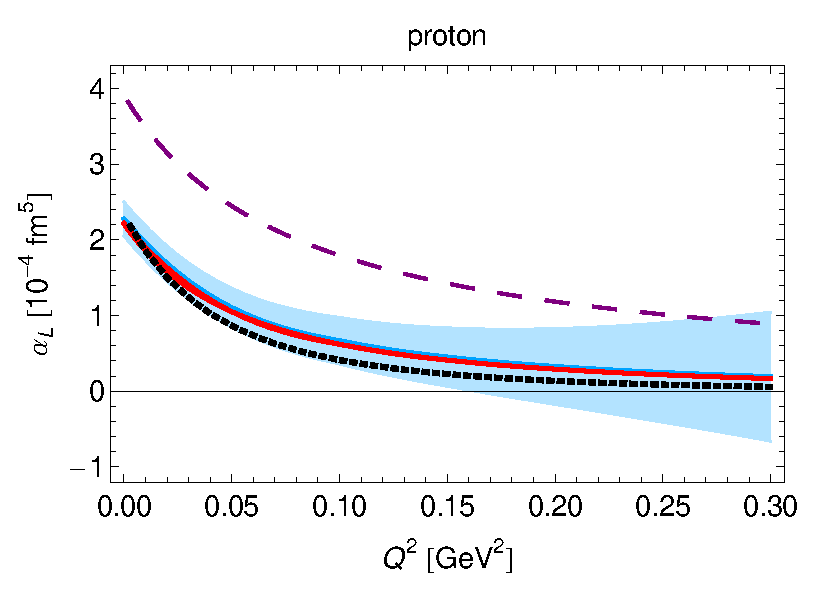
\epsfig{file=alphaL_p.eps,width=6.5cm,angle=0}\hspace{0.5cm}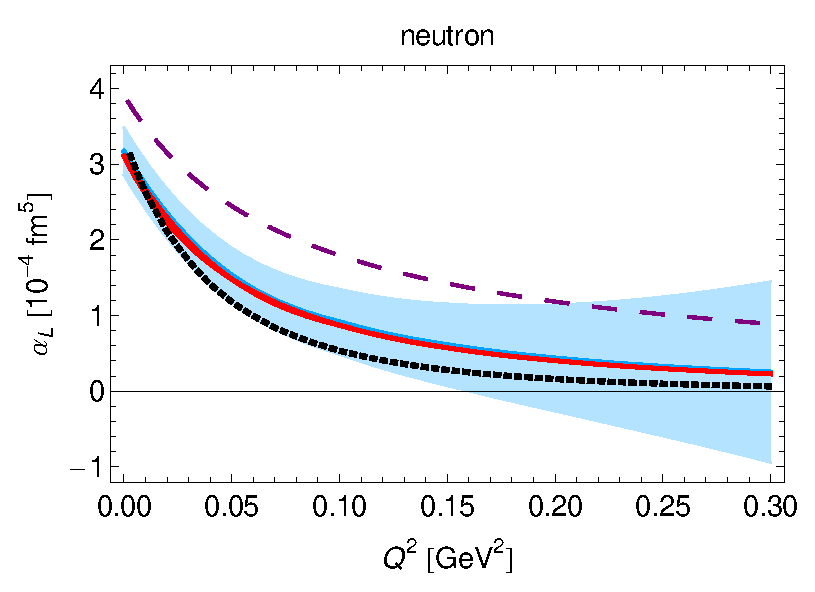
\epsfig{file=alphaL_n.eps,width=6.5cm,angle=0}
\caption{Longitudinal polarizability, $\alpha_L (Q^2)$, for the proton  (p) and neutron (n) as function of $Q^2$. The legend is the same as in Fig.~\ref{Fig:alpha+betaplot} except for the black dotted line which correspond to the MAID model prediction using only the $\pi$-channel \cite{Drechsel:2002ar}.  \label{Fig:alphaLplot}}
\end{center}
\end{figure}

The longitudinal polarizability,
\beq
\alpha_L (Q^2)= \frac{1}{2 \pi^2} \int_{\nu_0}^\infty\! \dd\nu'\, \frac{K(\nu',Q^2)}{\nu'}              \frac{\sigma_L (\nu',Q^2)}{Q^2\, \nu'^2} = \frac{4 \al M_N}{Q^6}\int_0^{x_0}\! \dd x \, f_L(x,Q^2),\label{Eq:alphaLQ2}
\eeq
with
\beq
f_L(x,Q^2)=-2xf_1(x,Q^2)+\left[1+\frac{4M_N^2 x^2}{Q^2}\right]f_2(x,Q^2),\nn
\eeq
provides information about the internal structure of the nucleon responding to longitudinaly polarized photons. 
It contributes to $T_2(\nu,Q^2)$ at $\mathcal{O}(Q^4)$, and therefore, is a  subleading structure correction to the (muonic-)hydrogen Lamb shift.

Our B$\chi$PT prediction for $\alpha_L(Q^2)$ is shown in Fig.~\ref{Fig:alphaLplot}, 
where we compare our results, with and without the Delta contributions, with the MAID model predictions~\cite{Drechsel:2000ct,Drechsel:1998hk,Drechsel:2002ar,private-Lothar} and the HB limit of the $\pi N$-loop contribution. One can see that the Delta plays a negligible role in the low-$Q^2$ evolution of $\alpha_L$, which in the B$\chi$PT approach is dominated by $\pi N$ loops.
Our results run very close to the MAID curves, with small discrepancies in the intermediate $Q^2$ region.
At higher virtualities, these discrepancies decrease.
The HB approach, on the other hand, seems to systematically overestimate the value of $\alpha_L$ in the considered $Q^2$ range. 
This relatively big mismatch, very similar to the discrepancy observed in HB calculations of $\delta_{LT}^n$, can be traced back to the slow convergence of the $1/M_N$ expansion, as one can see from the analytic expression for the $\pi N$-loop contribution to $\alpha_L(Q^2=0)$ given in  Appendix~\ref{App:Polarizabilities}.  As in the case of $\delta_{LT}^n$, this systematic deviation is cured in the relativistic formulation. 

For the static values of $\alpha_L$,
we obtain the following contributions from $\pi N$ loops,  $\Delta$ exchange and $\pi\Delta$ loops, in units of $10^{-4}$~fm$^5$:
\begin{align}
\alpha^p_L=2.28(22)\approx 2.22+ 0.00+  0.06, \\
\alpha^n_L= 3.17(31)\approx 3.11 + 0.00+ 0.06.
\end{align}
For the slopes at $Q^2=0$, we find, in units of $10^{-4}$~fm$^7$:
\begin{align}
\left.\frac{\dd\alpha^p_L (Q^2)}{\dd Q^2}\right|_{Q^2=0}&=-1.63(16)\approx  -1.62 + 0.01 - 0.01  ,  \\
\left.\frac{\dd\alpha^n_L (Q^2)}{\dd Q^2}\right|_{Q^2=0}&= -2.25(22)\approx -2.24 + 0.01 - 0.01.
\end{align}
 The corresponding individual contributions to the $Q^2$ dependence
of $\alpha_L(Q^2)$ are demonstrated in Fig.~\ref{Fig:alphaL-orders}. One again notices
that  $\Delta$ exchange and  $\pi \Delta$ loops give negligible contributions in this $Q^2$ range, with the $\Delta$-exchange contribution being even smaller than the $\pi \Delta$-loop contribution. 
The latter feature is explained by the fact that the magnetic coupling $g_M$ does not contribute to $\al_L$.







\section{Summary and conclusions}\label{Sec:Summary}

%\textcolor{red}{Vadim: Could you please mention the "to be published" JLab results or other experimental programs related to the spin structure? I'm a bit disconnected from all that.}

\begin{table}[h]
\caption{The NLO B$\chi$PT predictions for the forward VVCS polarizabilities at $Q^2=0$. The contributions of the $\pi N$ loops, the $\Delta$ exchange and the $\pi\Delta$ loops are shown, together with the combined total NLO predictions.
\label{Table:Individual-Results-Pol}}
\begin{tabular}{cc|c|c|c|c|}
\cline{3-6} 
&& $\pi N$ loops & $\Delta$ exchange   & $\pi\Delta$ loops & Total \\
\hline
\multicolumn{1}{|c||}{$\alpha_{E1}+\beta_{M1}$} &$p$&$5.10$&$\hpm7.04$&$\hpm2.98$&$\hpm15.12(1.48)$\\
\multicolumn{1}{|c||}{$(10^{-4}$~fm$^3)$} &$n$&$8.28$&$\hpm7.04$&$\hpm2.98$&$\hpm18.30(1.79)$\\
\hline
\multicolumn{1}{|c||}{$\alpha_L$}&$p$ &$2.22$&$\hpm0.00$&$\hpm0.06$&$\hpm2.28(22)$\\
\multicolumn{1}{|c||}{$(10^{-4}$~fm$^5)$} &$n$&$3.11$&$\hpm0.00$&$\hpm0.06$&$\hpm3.17(31)$\\
\hline
\end{tabular}
\end{table}






\begin{table}[h]
\caption{The NLO B$\chi$PT predictions for the forward VVCS polarizabilities at $Q^2=0$,
compared with the available empirical information. Where the reference is
not given, the empirical number is provided by the MAID analysis \cite{Drechsel:2000ct,MAID} with unspecified uncertainty.
\label{Table:Results-Pol}}
\begin{tabular}{c|c|c||c|c|}
\cline{2-5} 
&  \multicolumn{2}{|c||}{ Proton} & 
\multicolumn{2}{|c|}{Neutron} \\
\cline{2-5} 
  & \, This work \, & Empirical   & \, This work\, & \,\,Empirical\,\, \\
\hline
\multicolumn{1}{|c|}{$\alpha_{E1}+\beta_{M1}$} &$\hpm15.12(1.48)$ & $13.8(4)$ &$18.30(1.79)$  &$14.40(66)$\\
\multicolumn{1}{|c|}{$(10^{-4}$~fm$^3)$} & & Ref.~\cite{Olm01}& &Ref.~\cite{Babusci:1997ij}\\
\hline
\multicolumn{1}{|c|}{$\alpha_L$} &$\hpm2.28(22)$ & $2.32$ & $3.17(31)$  & $3.32$\\
\multicolumn{1}{|c|}{$(10^{-4}$~fm$^5)$} &&[MAID]&&[MAID]\\
\hline
\end{tabular}
\end{table}

\begin{table}[h]
\caption{The NLO B$\chi$PT predictions for the derivatives of the moments of the nucleon structure functions at $Q^2=0$. The contributions of the $\pi N$ loops, the $\Delta$ exchange and the $\pi\Delta$ loops are shown, together with the combined total NLO predictions. 
\label{Table:Results-DerPol}}
\begin{tabular}{cc|c|c|c|c|}
\cline{3-6} 
&& $\pi N$ & $\Delta$ exchange   & $\pi\Delta$ &  Total \\
\hline
\multicolumn{1}{|c||}{$(\alpha_{E1}+\beta_{M1})'$} &$p$&$-0.74$&$\hpm0.74$&$-0.20$&$-0.19(6)$\\
\multicolumn{1}{|c||}{$(10^{-4}$~fm$^5)$} &$n$&$-1.22$&$\hpm0.74$&$-0.20$&$-0.68(21)$\\
\hline
\multicolumn{1}{|c||}{$(\alpha_L)'$}&$p$ &$-1.62$&$\hpm0.01$&$-0.01$&$-1.63(16)$\\
\multicolumn{1}{|c||}{$(10^{-4}$~fm$^7)$} &$n$&$-2.24$&$\hpm0.01$&$-0.01$&$-2.25(22)$\\
\hline
\end{tabular}
\end{table}


In this article, we have computed a NLO parameter-free prediction of the scalar and spin polarizabilities, as well as some other moments of the proton and neutron structure functions for finite $Q^2$ in covariant B$\chi$PT. 
We calculated the VVCS amplitudes at N$^2$LO including explicitly the contribution of the $\Delta(1232)$ as an intermediate state with a dipole form factor for its magnetic coupling. The later turns out to be very important in the descriptions of the sum of electric and magnetic dipole polarizabilities $\alpha_{E1}+\beta_{M1}$, which indicates the importance of including vector-meson exchanges in $\chi$PT to account properly for the $Q^2$ behavior of the polarizabilities. We found that the Delta plays a fundamental role in the description of the $Q^2$ dependence of $\alpha_{E1}+\beta_{M1}$, but basically no role in the longitudinal polarizability $\alpha_L$. The Coulomb coupling, $g_C$, on the other hand didn't play a relevant role in the scalar polarizabilities, while the $\pi\Delta$ loops were relevant only for $\alpha_{E1}+\beta_{M1}$.

In general, we obtain a good description of the $Q^2$ evolution of the polarizabilities and the moments of the structure functions, improving the previous $\chi$PT predictions.
In this regard, we compared our calculation to the HB approach \cite{Nevado:2007dd}, as well as to the MAID model prediction \cite{MAID}. 
It is shown that in our approach we obtain results which are closer to  MAID than the HB calculation.

We also proved the validity of the sum rules for $\alpha_{E1}+\beta_{M1}$ and $\alpha_L$ at LO in $\chi$PT for arbitrary $Q^2$:
Evaluating the sum rules with the $\mathcal{O}(p)$  pion electroproduction cross sections, we were able to reproduce the $\mathcal{O}(p^3)$ results for the polarizabilities and moments obtained directly from forward VVCS in covariant $\chi$PT.
We give analytic expressions for the relativistic predictions of the $\pi N$-loop and $\Delta$-exchange contributions to the static polarizabilities and moments, as well as their slopes, see Appendix~\ref{App:PolarizabilitiesAll}.
For some polarizabilities, such expansions are given for first time in the literature. 
The contribution of the $\pi \Delta$ loops is not shown due to the length of the  expressions.

We conclude that, in order to predict correctly the $Q^2$ evolution of the polarizabilities and the moments of the structure functions, it is important to combine three ingredients: the relativistic structure of the effective-field-theory calculation, the inclusion of the $\Delta(1232)$ excitation, and the effect of the vector-meson exchange.



\section*{Acknowledgements}

We thank Lothar Tiator and Marc Vanderhaeghen for helpful discussions. This work is supported by the Deutsche Forschungsgemeinschaft (DFG) through the
Collaborative Research Center [The Low-Energy Frontier of the Standard Model (SFB 1044)]. JMA acknowledges support from the Community of Madrid through the ``Programa de atracci\'on de talento investigador 2017 (Modalidad 1)'', and the Spanish MECD grants FPA2016-77313-P. FH gratefully acknowledges financial support from the Swiss National Science Foundation.



\appendix
\small

\section{Laboratory-frame decomposition of the VVCS amplitude}
\seclab{SRVVCStensor}
In the laboratory frame, the forward VVCS amplitude can be parametrized,
in terms of the nucleon Pauli matrices $\vec{\sigma}$, by four scalar functions $f_L$, $f_T$,
$g_{TT}$, and $g_{LT}$:
%\bea\label{Eq:T-Compt-definition}
%T(\nu,Q^2)&=&\eta\eta'\,f_{L}(\nu,Q^2) +(\vec{\epsilon}^{\,\, \prime *} \cdot \vec{\epsilon}\,) \,f_{T}(\nu,Q^2)  +  i \vec{\sigma}\cdot (\vec{\epsilon}^{\,\, \prime *} \times \vec{\epsilon}\,)\, g_{TT}(\nu,Q^2) \\
%&&-  i \vec{\sigma}\cdot [(\eta\,\vec{\epsilon}^{\,\, \prime *} - \vec{\epsilon}\,\eta')\times \hat{q}]\, g_{LT}(\nu,Q^2)\,.\nn 
%\eea
%This decomposition distinguishes between the longitudinal and transverse photons. Here, $\vec\epsilon$ ($\vec\epsilon^{\,\,\prime}$) is the incoming (outgoing) transverse photon polarization three-vector, $q$ is the photon four-momentum, $Q^2=-q^2$ is the virtuality of the photon and $\nu=(s-M_N^2+Q^2)/2M_N$ is the energy of the photon in the lab system.
%The coefficients $\eta$ and $\eta'$ correspond to the initial or final photon,
%respectively, and are equal to one (zero) if the photon is longitudinal (transverse).
\bea\label{Eq:T-Compt-definition}
T(\nu,Q^2)&=&\varepsilon_0\varepsilon_0^{\,\prime*}\,f_{L}(\nu,Q^2) +(\vec{\varepsilon}^{\,\, \prime *} \cdot \vec{\varepsilon}\,) \,f_{T}(\nu,Q^2)  +  i \vec{\sigma}\cdot (\vec{\varepsilon}^{\,\, \prime *} \times \vec{\varepsilon}\,)\, g_{TT}(\nu,Q^2) \\
&&-  i \vec{\sigma}\cdot [(\varepsilon_0\vec{\varepsilon}^{\,\, \prime *} - \vec{\varepsilon}\,\varepsilon^{\,\prime *}_0)\times \hat{q}]\, g_{LT}(\nu,Q^2)\,.\nn 
\eea
Here, $Q^2=-q^2$ is the virtuality of the photon with $q$ being the photon four-momentum, $\nu=(s-M_N^2+Q^2)/2M_N$ is the energy of the photon in the lab system, $\vec q$ and $\hat{q}=\vec{q}/\vert \vec{q}\, \vert$ are the photon three-momentum in the lab system and its unit vector. The modified polarization vector components are given by
\begin{align}
\varepsilon_0&=\left[\epsilon_0-\frac{\nu}{\left|\vec q\,\right|}\, (\vec\epsilon\cdot\hat q\,)\right]\frac{\left|\vec q\,\right|}{Q}\,,
&\vec\varepsilon = \vec\epsilon-\hat q\,(\vec\epsilon\cdot\hat q\,)\,,\eqlab{modified_polarization_vectors}
\end{align}
 where $\epsilon=(\epsilon_0,\vec\epsilon\,)$ is the usual photon polarization vector of the initial photon; the primed
polarization vectors and their components  correspond to the final photon.

Two of the scalar VVCS amplitudes are independent of the spin ($f_T$ and $f_L$), while the other two ($g_{TT}$ and $g_{LT}$) are spin dependent. 
In the real-photon case ($Q^2=0$), the amplitudes involving a longitudinally polarized  photon ($f_L$ and $g_{LT}$) vanish, and only $f_T$ and $g_{TT}$ survive. 
Low, Gell-Mann and Goldberger \cite{ Low:1954kd, Gell_Mann:1954kc} proved that the leading terms of the LEX of these amplitudes are determined uniquely by the global properties of the nucleon: charge, mass and anomalous magnetic moment. 
The polarizabilities, related to the internal structure of the nucleon, enter as higher-order corrections, and are accessible through photoabsorption experiments (see Appendix~\ref{App:CrossSections}).



%\columnbreak
Constructed from crossing symmetry, Lorentz and gauge invariance, the spin-independent functions have the general structures: 
\begin{subequations}
\eqlab{fgFunctions}
\begin{eqnarray}
  f_T(\nu, Q^2))&=& f_T^{\mathrm{Born}}(\nu, Q^2)+4\pi\left[ Q^2 \beta_{M1}(Q^2) +(\alpha_{E1}(Q^2) + \beta_{M1}(Q^2)) \nu^2\right] + \dots \label{Eq:LEX-fT}\\
  f_L(\nu, Q^2)&=& f_L^{\mathrm{Born}}(\nu, Q^2) + 4 \pi\left[\alpha_{E1}(Q^2)+\alpha_{L}(Q^2) \nu^2\right] Q^2 + \dots \qquad \label{Eq:LEX-fL}\\
%  g_{TT}(\nu, Q^2)&=&g^{\mathrm{Born}}_{TT}(\nu, Q^2) + 4 \pi\gamma_0(Q^2)  \nu^3 + \dots \label{Eq:LEX-gTT}\\
 % g_{LT}(\nu, Q^2)&=&g^{\mathrm{Born}}_{LT}(\nu, Q^2) +  4 \pi\delta_{LT}(Q^2) \nu^2 Q + \dots \label{Eq:LEX-gLT}
\end{eqnarray}
\end{subequations}
where the Born terms are \cite{Drechsel:2002ar}:
\begin{subequations}
\begin{align}
 & f_T^{\mathrm{Born}}(\nu, Q^2) =  - \frac{4\pi \alpha}{M_N} \Big( F_1^2 + \frac{\nu_B^2 G_M^2}{\nu^2-\nu_B^2} \Big), \label{Eq:BT-fT}\\
  &  f_L^{\mathrm{Born}}(\nu, Q^2) = - \frac{\pi \alpha Q^2}{ M_N^3} \Big( F_2^2 + \frac{4M_N^2 G_E^2}{\nu^2-\nu_B^2} \Big), \label{Eq:BT-fL}\\
% & g^{\mathrm{Born}}_{TT}(\nu, Q^2) = - \frac{2\pi \alpha \nu}{ M_N^2} \Big( F_2^2 + \frac{Q^2 G_M^2}{\nu^2-\nu_B^2} \Big), \label{Eq:BT-gTT}\\
% & g^{\mathrm{Born}}_{LT}(\nu, Q^2) =  \frac{2 \pi\alpha Q}{M_N^2} \Big( F_1 F_2 - \frac{Q^2 G_E G_M }{\nu^2-\nu_B^2} \Big), \label{Eq:BT-gTL}
\end{align}
\end{subequations}
with $G_E(Q^2)$ and $G_M(Q^2)$ the electric and magnetic Sachs form factors, and $\nu_B=Q^2/2M_N$. 
The Sachs form factors are related to the Dirac and Pauli form factors in the following way:
\begin{subequations}
\begin{align}
& G_E(Q^2)=F_1(Q^2) - \frac{Q^2}{4M_N^2} F_2(Q^2),\\
& G_M(Q^2)=F_1(Q^2) + F_2(Q^2).
\end{align}
\end{subequations}


The polarizabilities in the  $\nu$ expansion of \Eqref{fgFunctions} are $Q^2$-dependent functions.
They  are the so-called generalized polarizabilities, which generalize the response of the nucleon to the case of finite momentum transfer. Notice that $\alpha_L$ is usually defined including the $Q^2$ proportionality that stems from gauge invariance. 
In this case, we think it is more natural to take $Q^2$ out of the definition, as is usually done with $Q$ in $\delta_{LT}$.



In order to extract the generalized polarizabilities, it will be useful to keep in mind the relation between the explicitly covariant \eqref{Eq:T-Rel} and the lab-frame forms \eqref{Eq:T-Compt-definition}:
\begin{subequations}
\begin{align}
  f_T(\nu,Q^2) &= T_1(\nu,Q^2), \label{Eq:fT-T1}\\
  f_L(\nu,Q^2) &= - T_1(\nu,Q^2) +  \frac{\nu^2 + Q^2}{Q^2} T_2(\nu,Q^2), \label{Eq:fL-T1T2}\\
% g_{TT}(\nu, Q^2) &= \frac{\nu}{M_N}\Big[ S_1(\nu,Q^2) - \frac{Q^2}{M_N\,\nu} S_2(\nu,Q^2)\Big],\label{Eq:gTT-S1S2}\\
 % g_{LT}(\nu, Q^2) &= \frac{Q}{M_N}\Big[ S_1(\nu,Q^2) + \frac{\nu}{M_N} S_2(\nu,Q^2)\Big].\label{Eq:gLT-S1S2}
\end{align} 
\end{subequations}
The polarizabilities can then be obtained from linear combinations of the non-Born functions $\ol T_1$ and $\ol T_2$. 


%\subsection{Connection between forward Compton scattering and electroproduction}
%\label{Sec:ConnectionWithElectroproduction}


 

%In fact, Eqs.~\eqref{Eq:ImfTRealPhoton} and \eqref{Eq:ImgTTRealPhoton} imply that the coefficients in the expansions \eqref{Eq:LEX-fT} and \eqref{Eq:LEX-gTT},  i.e., the polarizabilities, can be determined from the experimental photoabsorption cross sections through a dispersive representation.
%In the real photon case, one recovers the well-known Baldin and FSP sum rules:
% \begin{align}
%\alpha_{E1}+\beta_{M1}&= \frac{1}{2 \pi^2} \int_{\nu_0}^\infty\! \dd\nu'\, \frac{\sigma_T (\nu')}{\nu'^2},\\
%\gamma_0&= \frac{1}{2 \pi^2} \int_{\nu_0}^\infty\! \dd\nu'\, \frac{\sigma_{TT} (\nu')}{\nu'^3}.
%\end{align}

%In the generalization to arbitrary virtualities, one finds two new polarizabilities at order $\nu^2$ which were absent at $Q^2=0$.
%These are the longitudinal polarizability $\alpha_L(Q^2)$ and the longitudinal-transverse polarizability $\delta_{LT}(Q^2)$. 
%Therefore, the generalization to finite $Q^2$ for the lowest-order polarizabilities leads to,
%\begin{align}
%[\alpha_{E1}+\beta_{M1}] (Q^2) &= \frac{1}{2 \pi^2} \int_{\nu_0}^\infty \! \dd\nu'\,\frac{K(\nu',Q^2)}{\nu'} \frac{\sigma_T (\nu',Q^2)}{\nu'^2}\\
%\gamma_0 (Q^2) &= \frac{1}{2 \pi^2} \int_{\nu_0}^\infty \! \dd\nu'\,\frac{K(\nu',Q^2)}{\nu'} \frac{\sigma_{TT} (\nu',Q^2)}{\nu'^3}
%\end{align}


%where $\nu_0=m_\pi + (m_\pi^2+Q^2)/2M_N$ is the value of $\nu$ at the inelastic threshold.
%On the other hand, the cross section for longitudinally polarized photons is defined as $\sigma_L=\half\, (\sigma_{1/2}+\sigma_{-1/2})$, while $\sigma_{LT}$ is the longitudinal-transverse cross section which involves a spin-flip of the nucleon, as described in Appendix~\ref{App:Extracting-SigmaLT}.

% and the definitions for the partial cross sections $\sigma_T$, $\sigma_L$, $\sigma_{TT}$ and $\sigma_{LT}$, can be found in \cite{Drechsel:2002ar,Drechsel:1992pn}. 



%\section{Convention for the flux factor $K$} \label{App:FluxFactor}



%The flux factor, $K$, introduced in Section \ref{Sec:ConnectionWithElectroproduction}, computes the flux of incoming particles in the initial state of the photoabsorption process. 
%It has been argued in different works that it is arbitrary since, in the electroproduction process, the measured cross section is proportional to $K\cdot \sigma_i$, where $\sigma_i$ are the partial cross sections defined in Refs.~\cite{Drechsel:2000ct, Drechsel:2002ar} ($\sigma_i=\sigma_T,\sigma_{TT},\sigma_L,\sigma_{LT}$ in our case). 
%Although this is correct, it is important to stress that this does not mean that one can use the Hand's \cite{Hand:1963bb}  or Gilman's \cite{Gilman:1967sn}  flux factors arbitrarily for a given cross section. On the contrary, one {\itshape must}  use the same flux factor as is used to calculate the cross sections.   
% This is seen clearly through to the optical theorem. Applied to our particular case, it states that:
%\begin{widetext}
%\begin{align}\label{Eq:AppA-1}
%&- i \mathcal{T}_{i\to i } + i \mathcal{T}_{i\to i }^*= \int\! \frac{d^3 k_1 }{(2\pi)^3 2E_1} \frac{d^3 k_{2} }{(2\pi)^3 2E_{2}} (2\pi)^4 \delta^4 (\mathcal{P}_\mathrm{incl} - \mathcal{P}_i) \mathcal{T}_{\alpha \to i}  \mathcal{T}_{\alpha \to i}^* \,,
%\end{align}
%\end{widetext}
%where $\mathcal{P}_{i}$ and $\mathcal{P}_\mathrm{incl}$ refer to the sum of the four-momenta in the initial state of the forward CS and the inclusive photoabsorption process, respectively. $\mathcal{T}= \bar{u}'_{h'} T u_h,$ are the scattering amplitudes including Dirac spinors.
%The standard form of the optical theorem is recovered once one relates the right-hand side of Eq.~\eqref{Eq:AppA-1}, which is the sum over the phase space, to the cross section, which is the sum over the phase space divided by the flux of the incoming particles in the initial state:
%\begin{align}%\label{Eq:AppA-2}
% \int\! \frac{\dd^3 k_1 }{(2\pi)^3 2E_1} \frac{\dd^3 k_{2} }{(2\pi)^3 2E_{2}} (2\pi)^4 \delta^4 (\mathcal{P}_\mathrm{incl} - \mathcal{P}_i) |\mathcal{T}|^2 = K\cdot \sigma. \qquad\;\nn
%\end{align}
%Then, what is relevant in the electroproduction processes is the sum over the phase space of the inclusive process.
%But to recover this sum over the phase space, it is mandatory that one uses the same flux factor used to calculate the cross section. 
%Therefore, in the application of the sum rules, the flux factor $K$ {\itshape must} be the same as the one used in the calculation of $\sigma$.
%In this way, one obtains the sum over the phase space of the inclusive process, which is what is related to the imaginary part of the forward process.

%In our case, since we consider the incident flux of virtual photons in the calculation of the cross sections, we had to use the Gilman's flux factor $K_G(\nu,Q^2)=|\vec{q}_i|_\mathrm{lab}$, where  $|\vec{q}_i|_\mathrm{lab}$ is the modulus of the three-momentum of the photon in the laboratory frame. See Ref.~\cite{Drechsel:2002ar} for common choices for the photon flux factor.

%If the flux factor used to calculate the cross section is the one corresponding to real photons (Hand's) $K_H$, is this the flux factor that must be used. But if it was the one corresponding to virtual photons (Gilman's) $K_G$ is then this flux factor the one that must enter in the dispersive calculation.



\section{Pion electroproduction cross sections}\label{App:CrossSections}

In the forward kinematics, the optical theorem allows us to reconstruct the Compton amplitude from the total photoabsorption cross sections. 
In the real-photon case, the imaginary parts of the surviving scalar functions, $f_T$ and $g_{TT}$, are related to the photoabsorption cross sections. 
The spin-independent one, $f_T$, is related to  $\sigma_T$ in the following way:
\begin{subequations}
\begin{align}
\text{Im}\, f_T(\nu, 0)&= K(\nu)\, \sigma_T(\nu), \label{Eq:ImfTRealPhoton}\\
%\text{Im}\,  g_{TT}(\nu, 0)&=K(\nu)\, \sigma_{TT}(\nu).\label{Eq:ImgTTRealPhoton}
\end{align}
\end{subequations}
Here, $K(\nu)$ is the flux factor of incoming photons which, for  real photons, is just the lab-frame energy of the incoming photon.

\begin{figure*}
\begin{center}
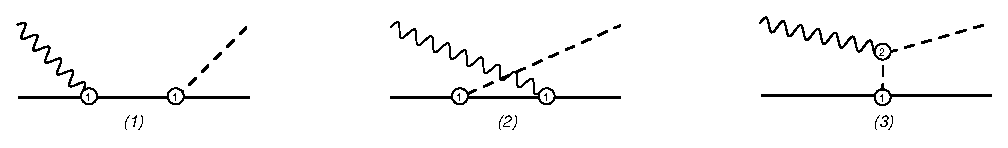
\epsfig{file=TreeLevelOp.eps,width=16cm,angle=0} 
\caption{Diagrams entering our calculation of the pion electroproduction amplitude at leading order. The numbers in the vertices indicate their chiral order.\label{Fig:DiagsOp}}
\end{center}
\end{figure*}

For the calculation of the cross sections, we compute the pion electroproduction amplitude in B$\chi$PT at LO.
We follow Refs.~\cite{Holstein:2005db,Lensky:2009uv} and perform a chiral rotation to cancel exactly the Kroll-Ruderman term at this order.
This means that we have to consider only the diagrams shown in Fig.~\ref{Fig:DiagsOp}, which are gauge invariant by themselves.

Decomposing the amplitude in the following way:
\begin{align}\label{Eq:T-decomposition}
\mathcal{T}= \bar{u}'_{h'} \sum_{i}  \mathcal{A}_i (s,t) \Gamma_i u_h,
\end{align}
where the Dirac structures are defined as:
\begin{align}\label{Eq:DefGammas}
  \Gamma_1&= \gamma_5, \\
  \Gamma_2&= \frac{1}{2}\left[\slashed{q}_A,\slashed{\epsilon}\right]\gamma_5,  
\end{align}
we obtain the following results for the different channels:
\begin{itemize}
 \item $\gamma^* p \to \pi^0 p$
\end{itemize}
\begin{align}
  &\mathcal{A}_1= \frac{e\, g_A M_N}{f_\pi}\left[\frac{2 P_A\cdot \epsilon + q_A\cdot \epsilon}{s-M_N^2} + \frac{2 P_B\cdot \epsilon - q_A\cdot \epsilon}{u-M_N^2}\right], \\
   &\mathcal{A}_2=\frac{e\, g_A M_N}{f_\pi}\left[\frac{1}{s-M_N^2} + \frac{1}{u-M_N^2}\right];
\end{align}


\begin{itemize}
 \item $\gamma^* p \to \pi^+ n$
\end{itemize}
\begin{align}
  &\mathcal{A}_1= \frac{\sqrt{2}\, e\, g_A M_N}{f_\pi}\left[\frac{2 P_A\cdot \epsilon + q_A\cdot \epsilon}{s-M_N^2} + \frac{2 (P_A - P_B)\cdot \epsilon + q_A\cdot \epsilon}{t-m_\pi^2}\right],\\
   &\mathcal{A}_2=\frac{\sqrt{2}\, e\, g_A M_N}{f_\pi(s-M_N^2)};
\end{align}


\begin{itemize}
 \item $\gamma^* n \to \pi^0 n$
\end{itemize}
\begin{align}
  &\mathcal{A}_1= 0,\\
  & \mathcal{A}_2=0;
\end{align}


\begin{itemize}
 \item $\gamma^* n \to \pi^- p$
\end{itemize}
\begin{align}
  &\mathcal{A}_1= \frac{\sqrt{2}\, e\, g_A M_N}{f_\pi}\left[\frac{2 P_B\cdot \epsilon - q_A\cdot \epsilon}{u-M_N^2}  - \frac{2 (P_A - P_B)\cdot \epsilon + q_A\cdot \epsilon}{t-m_\pi^2}\right],\\
   &\mathcal{A}_2=\frac{\sqrt{2}\, e\, g_A M_N}{f_\pi(u-M_N^2)};
\end{align}
They are written in terms of the four-momentum of the incoming (outgoing) nucleon $P_A$ ($P_B$), the incoming photon $q_A$, the outgoing pion $q_B$, the polarization vector of the photon $\epsilon$, the Mandelstam variables $s$, $t$ and $u$, the nucleon mass $M_N$, the pion mass $m_\pi$, the electron charge $e=\sqrt{4\pi \alpha}$, the nucleon axial coupling $g_A$, the pion weak decay constant $f_\pi$ and $\mu=m_\pi/M_N$. 
The analytical expressions shown above were checked with the amplitudes given in Ref.~\cite{Pasquini:2007fw}.



To shorten the final expressions, which are considerably longer for finite $Q^2$ than in the real-photon limit, we define the following dimensionless kinematic variables:
\begin{align}
&\alpha_\gamma= (E_i^{N})_\mathrm{cm}/\sqrt{s}=\frac{s+M_N^2+Q^2}{2 s},   \\
&\alpha_\pi= (E_f^{N})_\mathrm{cm}/\sqrt{s} = \frac{s+M_N^2-m_\pi^2}{2 s},  \\              
 & \beta_\gamma = E^{\gamma}_\mathrm{cm}/\sqrt{s} = \frac{s-M_N^2-Q^2}{2 s} ,  \\
 & \beta_\pi= E^{\pi}_\mathrm{cm}/\sqrt{s} = \frac{s-M_N^2+m_\pi^2}{2 s} , \\
 &\lambda_\gamma  = |\vec{q}_i|_\mathrm{cm}/\sqrt{s}= \frac{\sqrt{(s-M_N^2 - Q^2)^2+4 s Q^2}}{2 s},  \\
&\lambda_\pi =  |\vec{q}_f|_\mathrm{cm}/\sqrt{s}  = \frac{\sqrt{(s-M_N^2 + m_\pi^2)^2-4 s m_\pi^2}}{2 s}.  \end{align} 
Here, $(E_i^{N})_\mathrm{cm}$  and $(E_f^{N})_\mathrm{cm}$ are the energies of the incoming and outgoing nucleon, $E^{\gamma}_\mathrm{cm}$ is the energy of the incoming photon, $E^{\pi}_\mathrm{cm}$ is the energy of the outgoing pion, and $|\vec{q}_i|_\mathrm{cm}$ ($|\vec{q}_f|_\mathrm{cm}$) is the relative three-momentum of the incoming (outgoing) particles, all in the center-of-mass frame (cm).




%\subsection{Calculating $\sigma_{LT}$}
%\label{App:Extracting-SigmaLT}




Analytical expressions for the cross sections of the different pion electroproduction channels are listed below. 
We  checked that they reproduce the known results in the real-photon limit \cite{Lensky:2009uv,Holstein:2005db}.
These cross sections were also used to verify that the dispersion relations in \Eqref{genDRs} are satisfied in B$\chi$PT. We checked that the non-Born VVCS amplitudes at leading order, the left-hand side of \Eqref{genDRs}, are reproduced by the right-hand side of the same equation when the pion electroproduction cross sections from Appendix~\ref{App:CrossSections} are inserted \cite{Alarcon:2013cba}.

%\begin{widetext}




\subsection{Proton cross sections}



\begin{flalign}
\sigma_T^{(\pi^+ n)}=&\,\frac{e^2 g_A^2  M_N^2 \lambda_\pi}{32\pi f^2_\pi s^3 \lambda_\gamma^4} \left( \frac{2 s \lambda_\gamma}{(s-M_N^2)^2}\left\{ 2 M^2_\pi[(s-m^2_N)^2-Q^2 s \lambda_\gamma^2] + (M_N^2-s)[Q^4+2Q^2 s \beta_\gamma \beta_\pi \right.  \nonumber \right.&&\\
& \left.+ 2 s (M_N^2 -s+2 s \beta_\gamma \beta_\pi) \lambda_\gamma^2]\right\}+\frac{1}{(s-M_N^2)\lambda_\pi} \left\{  2 m_\pi^2 (M_N^2-s) (Q^2+2 s \beta_\gamma \beta_\pi) \right.\nonumber &&\\
&\left.\left.+Q^2[(Q^2+2 s\beta_\gamma \beta_\pi)^2-4 s^2 \lambda_\pi^2 \lambda_\gamma^2] \right\} \arctan\left[ \frac{2 s \lambda_\pi \lambda_\gamma}{Q^2 + 2 s \beta_\gamma \beta_\pi} \right]\right)  &&
\end{flalign}


\begin{flalign}
\sigma_T^{(\pi^0 p)}=&\frac{e^2 g_A^2 M_N^2 \lambda_\pi}{16 \pi f_\pi^2 s (s-M_N^2)^2 \lambda_\gamma} \Bigg\{ \frac{1}{-2 s(M_N^2 + s (-1 + 2 \beta_\gamma \beta_\pi))^2 \lambda_\gamma^2 + 8 s^3 \lambda_\pi^2 \lambda_\gamma^4}\big\{ (M_N^2 - s)[Q^2 (s \nonumber&&\\
&-M_N^2 -2 s \beta_\gamma \beta_\pi )- 2 s (s-M_N^2 + 2 s \beta_\gamma \beta_\pi) \lambda_\gamma^2] \{[M_N^2+s (-1 + 2 \beta_\gamma \beta_\pi)]^2 - 4 s^2 \lambda_\pi^2 \lambda_\gamma^2\} \nonumber&&\\
&+ 2 m_\pi^2 (-(s-M_N^2)^2 (M_N^2 + s(-1 + 2 \beta_\gamma \beta_\pi))^2 + 2 s (Q^2 (M_N^4 + 2 M_N^2 s(-1 + \beta_\gamma \beta_\pi) \nonumber &&\\ 
&+ s^2 (1 + 2 \beta_\gamma \beta_\pi (-1 + \beta_\gamma \beta_\pi))) + 2 (s-M_N^2)^2 s \lambda_\pi^2 )\lambda_\gamma^2 -4 Q^2 s^3 \lambda_\pi^2 \lambda_\pi^4 ) \big\}  \nonumber &&\\
&+ \frac{1}{4 s^2 \lambda_\pi \lambda_\gamma^3}(M_N^2-s) \left[-((2 m_\pi^2 +Q^2)(M_N^2 - s) + 2 Q^2 s \beta_\gamma \beta_\pi)(M_N^2+s(-1+2 \beta_\gamma \beta_\pi))\right.\nonumber&& \\
&\left.+2s (M_N^4 - 2 M_N^2 s +s^2 + 2 Q^2 (m_\pi^2 + s \lambda_\pi^2))\lambda_\gamma^2\right]\arctan\left[ \frac{2 s \lambda_\pi \lambda_\gamma}{M_N^2 + s (-1 + 2 \beta_\gamma \beta_\pi)}\right]\Bigg\}&&
\end{flalign}

\begin{flalign}
\sigma_{L}^{(\pi^+ n)}=&\,\frac{e^2 g_A^2 M_N^2 \lambda_\pi}{16 \pi f_\pi^2 Q^2 \, s (s-M_N^2)^2 \lambda_\gamma^4}\left\{   \frac{1}{(Q^2 + 2 s \beta_\gamma \beta_\pi )^2 - 4 s^2 \lambda_\pi^2 \lambda_\gamma^2}    \left[ 2 \lambda_\gamma (-Q^2(M_N^2-s) \right.\right.\nonumber&&\\
& \times(\beta_\gamma^2 (Q^2+2 s \beta_\gamma \beta_\pi) + (M_N^2 + s (-1 +  \beta_\gamma(-1 + 2 \alpha_\pi+ \beta_\pi)))   \lambda_\gamma^2)   ((Q^2+2 s \beta_\gamma \beta_\pi)^2  \nonumber &&\\
& - 4 s^2 \lambda_\pi^2 \lambda_\gamma^2) + m_\pi^2 (-2 (s-M_N^2)^2 \beta_\gamma^2 (Q^2+2s \beta_\gamma \beta_\pi)^2+ (Q^8 + 4 Q^6 s \beta_\gamma \beta_\pi \nonumber &&\\
&- 4 Q^2 (M_N^2 - s) s \beta_\gamma ((M_N^2-s)(-1+\alpha_\pi)+4 s \beta_\gamma \beta_\pi) + 4 Q^4 s \beta_\gamma (s  -M_N^2 + s \beta_\gamma \beta_\pi^2)  \nonumber &&\\
&+4 s^2 (s-M_N^2) \beta_\gamma^2  (2 \beta_\pi ((M_N^2 - s) (-1+\alpha_\pi) + 2 s \beta_\gamma \beta_\pi) + (s-M_N^2) \lambda_\pi^2) )\lambda_\gamma^2 \nonumber &&\\
&- 4 s^2 ((M_N^4 +s^2 )(\alpha_\pi^2-1)^2 + (Q^2 + 2 s \beta_\gamma \beta_\pi)^2 + (Q^4 + 4 s^2 \beta_\gamma) \lambda_\pi^2 - 2 M_N^2 s ((\alpha_\pi^2-1)^2\nonumber&&\\  &\left.+ 2 \beta_\gamma \lambda_\pi^2) )\lambda_\gamma^4+ 16 s^4 \lambda_\pi^2 \lambda_\gamma^6   )   ) \right]   + \frac{M_N^2 - s}{s\lambda_\pi}  \left[   \beta_\gamma (Q^2 + 2 s \beta_\gamma \beta_\pi) + 2 s (\alpha_\pi-1) \lambda_\pi^2    \right] \nonumber&&\\ &\times \left[  \beta_\gamma (Q^4 + 2 m_\pi^2 (M_N^2 - s) + 2 Q^2 s \beta_\gamma \beta_\pi  ) \right.\nonumber&&\\ 
&\left.\left.+ 2 s (2 m_\pi^2 + Q^2 \alpha_\pi) \lambda_\gamma^2     \right]      \arctan\left[ \frac{2 s \lambda_\pi \lambda_\gamma }{Q^2+ 2 s \beta_\gamma \beta_\pi}\right]  \right\} &&
\end{flalign}

\begin{flalign}
\sigma_{L}^{(\pi^0 p)}=&\,\frac{e^2 g_A^2 M_N^2 \lambda_\pi}{32 \pi f_\pi^2 Q^2\, s(s-M_N^2)^2 \lambda_\gamma^4}\Big\{  \frac{1}{(M_N^2+s(-1+2 \beta_\gamma \beta_\pi))^2 -4 s^2 \lambda_\pi^2 \lambda_\gamma^2}\big[  4m_\pi^2 \lambda_\gamma (-(M_N^2 -s )^2  \nonumber &&\\
 &\times\beta_\gamma^2 (M_N^2 + s (-1+2\beta_\gamma \beta_\pi))^2 + (-2 M_N^6 s (1+\alpha_\pi) \beta_\gamma + M_N^4 (Q^4 + 2 s^2 \beta_\gamma (3- 4 \beta_\gamma \beta_\pi \nonumber &&\\
 &+3\alpha_\pi  - 2 \alpha_\pi \beta_\gamma \beta_\pi + \beta_\gamma \lambda_\pi^2)) + s^2 (Q^4 (1+2 \beta_\gamma \beta_\pi (-1 + \beta_\gamma \beta_\pi)) + 2 s^2 \beta_\gamma (\alpha_\pi - 2\alpha_\pi \beta_\gamma \beta_\pi  \nonumber &&\\
 &+ \beta_\gamma \lambda_\pi^2) ) - 2+ (1-2 \beta_\gamma \beta_\pi)^2 M_N s (Q^4 (1-\beta_\gamma \beta_\pi) +s^2 \beta_\gamma (3+\alpha_\pi (3-4\beta_\gamma \beta_\pi) +2 \beta_\gamma  \nonumber&& \\
 &\times (2 \beta_\pi (\beta_\gamma \beta_\pi -2) + \lambda_\pi^2)))) \lambda_\gamma^2- 2 s^2 (M_N^4(1+\alpha_\pi^2) + Q^4 \lambda_\pi^2 - 2 M_N^2 s (1+\alpha_\pi^2 - 2 \beta_\gamma \beta_\pi  \nonumber &&\\
 &+ 2 \beta_\gamma \lambda_\pi^2) + s^2 (\alpha_\pi^2+(1-2 \beta_\gamma \beta_\pi)^2 + 4 \beta_\gamma \lambda_\pi^2)) \lambda_\gamma^4+ 8 s^4 \lambda_\pi^2 \lambda_\gamma^6)  - 2 Q^2 (M_N^2 - s) \lambda_\gamma (s \beta_\gamma^2  \nonumber &&\\
&\times (-1+2 \beta_\gamma \beta_\pi) + s (1+2 (-2 + 2 \alpha_\pi +\beta_\pi)) \lambda_\gamma^2 - (Q^2 M_N^2/s)) (M_N^2 +s (-1+ 2 \beta_\gamma \beta_\pi \nonumber&&\\
&- 2 \lambda_\pi \lambda_\gamma )) (M_N^2 + s(-1 +2 \beta_\gamma \beta_\pi+2 \alpha_\pi \alpha_\gamma))\big] +\frac{M_N^2-s}{s \lambda_\pi} \big[   2m_\pi^2 (-Q^4 \lambda_\gamma^2 +((M_N^2-s) \beta_\gamma  \nonumber &&\\
&+ 2 s \lambda_\gamma^2)(M_N^2 \beta_\gamma+ s \beta_\gamma(-1+2 \beta_\gamma \beta_\pi) +2 s \alpha_\pi \lambda_\gamma^2)) + Q^2 (M_N^2 (\beta_\gamma-\lambda_\gamma) + s (\beta_\gamma (2 \beta_\gamma \beta_\pi-1) \nonumber&& \\
& + \lambda_\gamma+2(\alpha_\pi -1)\lambda_\gamma^2  )) (M_N^2 (\beta_\gamma+\lambda_\gamma) + s (\beta_\gamma (-1+2 \beta_\gamma \beta_\pi) + \lambda_\gamma(-1+2 (\alpha_\pi-1)\lambda_\gamma) )  ) \big]\nn&&\\
&\times\arctan\Big[  \frac{2 s \lambda_\pi \lambda_\gamma}{M_N^2+ s (-1+2 \beta_\gamma \beta_\pi)} \Big]\Big\}&&
\end{flalign}


\subsection{Neutron cross sections}

\begin{flalign}
\sigma_T^{(\pi^0 n)}=&\,0&&
\end{flalign}

\begin{flalign}
\sigma_T^{(\pi^- p)}=&\,\frac{e^2 g_A^2 M_N^2}{64 \pi  f_\pi^2 \lambda _\pi^4 s^3(s-M_N^2+Q^2)}\Bigg\{4 (Q^2+2 \beta_\gamma  \beta_\pi 
   s) (m_\pi^2 (M_N^2+s (2 \beta_\gamma  \beta_\pi -1))-2\lambda_\pi^2 \lambda_\gamma^2 s^2)  \nonumber &&\\ 
   &\times \arctanh\left(\frac{2
   \lambda_\pi \lambda_\gamma s}{Q^2+2 \beta_\gamma  \beta_\pi s}\right)-\frac{1}{ (M_N^2+s (2\beta_\gamma  \beta_\pi -1))^2-4 \lambda_\pi^2 \lambda_\gamma^2 s^2}\Bigg[8 \lambda_\pi \lambda_\gamma m_\pi^2 s  \nonumber &&\\
   &\times  ((M_N^2+s (2 \beta_\gamma  \beta_\pi -1))^2  - \lambda_\gamma^2 s (Q^2+4 \lambda_\pi^2 s)) - (M_N^2+s (2 \beta_\gamma  \beta_\pi -2 \lambda_\pi
   \lambda_\gamma-1))  \nonumber &&\\
   & \times(M_N^2+s (2 \beta_\gamma  \beta_\pi +2 \lambda_\pi \lambda_\gamma-1)) \Big(-4 \lambda_\pi^2
   \lambda_\gamma^2 s^2 (-2 m_\pi^2+Q^2+2 \beta_\gamma  \beta_\pi  s\Big) \nonumber &&\\
   &\times \log \frac{(M_N^2+s (2 \beta_\gamma  \beta_\pi +2 \lambda_\pi
   \lambda_\gamma-1)) (Q^2+2 \beta_\gamma  \beta_\pi  s-2 \lambda_\pi \lambda_\gamma s)}{(M_N^2+s (2 \beta_\gamma  \beta_\pi -2
   \lambda_\pi \lambda_\gamma-1)) (Q^2+2 s (\beta_\gamma  \beta_\pi +\lambda_\pi \lambda_\gamma))} \nonumber &&\\
    &+2 \arctanh\left(\frac{2 \lambda_\pi \lambda_\gamma s}{M_N^2+s (2 \beta \gamma  \beta_\pi -1)}\right) ((M_N^2-Q^2-s)
   (M_N^2+s (2 \beta_\gamma  \beta_\pi -1))  \nonumber&& \\
   &\times (2 m_\pi^2+M_N^2+s(2 \beta_\gamma  \beta_\pi -1)) +2 \lambda_\gamma^2 s ((s-M_N^2) (M_N^2-Q^2-s)+2 \lambda_\pi^2 s (Q^2+2 \beta_\gamma  \beta_\pi  s)))\nonumber&& \\
   &-(2 m_\pi^2+M_N^2-Q^2-s) (M_N^2+s (2 \beta_\gamma  \beta_\pi
   -1))^2  \log \left(\frac{M_N^2+s (2 \beta_\gamma  \beta_\pi +2
   \lambda_\pi \lambda_\gamma-1)}{M_N^2+s (2 \beta_\gamma  \beta_\pi
   -2 \lambda_\pi \lambda_\gamma-1)}\right)\Bigg]\Bigg\}&&
\end{flalign}

\begin{flalign}
\sigma_{L}^{(\pi^0 n)}=&\,0&&
\end{flalign}

\begin{flalign}
\sigma_{L}^{(\pi^- p)}=&\,\frac{e^2 g_A^2 M_N^2 \lambda _{\pi }}{32
   \pi  Q^2 s f_{\pi }^2 \lambda _{\gamma }^4}  (-( \frac{4 \lambda _{\gamma }}{((Q^2+2 s \beta
   _{\pi } \beta _{\gamma }){}^2-4 s^2 \lambda _{\pi }^2 \lambda _{\gamma
   }^2) ((M_N^2+s (2 \beta _{\pi } \beta _{\gamma
   }-1)){}^2-4 s^2 \lambda _{\pi }^2 \lambda _{\gamma }^2)}  \nonumber &&\\
    & \times (-16 s^4
   (2 (\alpha _{\pi }-1) \alpha _{\pi }+1) \lambda _{\pi }^2
   \lambda _{\gamma }^6+4 s^2 ((\alpha _{\pi }^2+\lambda _{\pi }^2)
   Q^4+4 s \beta _{\gamma } (\beta _{\pi } \alpha _{\pi }^2-\lambda _{\pi }^2
     \alpha _{\pi }+\lambda _{\pi }^2) Q^2      \nonumber &&\\
   &  +s^2 ((4 \beta _{\pi } \beta 
   _{\gamma } (2 \beta _{\pi } \beta _{\gamma }-1)+1) \alpha _{\pi
   }^2-2 (1-2 \beta _{\pi } \beta _{\gamma }){}^2 \alpha _{\pi }+4 \beta
   _{\gamma } (1-4 \beta _{\pi } \beta _{\gamma }) \lambda _{\pi }^2 \alpha
   _{\pi } +4 \beta _{\pi } \beta _{\gamma } (2 \beta _{\gamma } \lambda _{\pi
      }^2  \nonumber &&\\
    & +\beta _{\pi } \beta _{\gamma }-1)+1)) \lambda _{\gamma}^4 -(Q^8+4 s \beta _{\pi } \beta _{\gamma } Q^6+4 s^2 \beta _{\gamma } (-2
   \beta _{\pi } \beta _{\gamma } \alpha _{\pi }+\alpha _{\pi }+\beta _{\gamma }
   (\beta _{\pi }^2+\lambda _{\pi }^2)) Q^4    \nonumber &&\\
   &  + 4 s^3 \beta _{\gamma }
   (-\alpha _{\pi } (2 \beta _{\pi } \beta _{\gamma }-1) (6 \beta
      _{\pi } \beta _{\gamma }-1)+4 \beta _{\pi } \beta _{\gamma } (\beta_{\gamma } (\lambda _{\pi }^2+\beta _{\pi })-1)+1) Q^2+4 s^4
   \beta _{\gamma }^2 (\lambda _{\pi }^2  \nonumber \\
   & +2 \beta _{\pi } (2 \beta _{\pi }
   \beta _{\gamma }-1) (-4 \beta _{\pi } \beta _{\gamma } \alpha _{\pi
   }+\alpha _{\pi }+2 \beta _{\gamma } (\lambda _{\pi }^2+\beta _{\pi
      })-1))) \lambda _{\gamma }^2 +2 s^2 \beta _{\gamma }^2
   (1-2 \beta _{\pi } \beta _{\gamma }){}^2 (Q^2   \nonumber &&\\
  & +2 s \beta _{\pi }
   \beta _{\gamma }){}^2+2 M_N^4 (2 s^2 (\alpha _{\pi }-1){}^2
   \lambda _{\gamma }^4+2 s \beta _{\gamma } ((\alpha _{\pi }-1)
   (Q^2+2 s \beta _{\pi } \beta _{\gamma })-s \beta _{\gamma } \lambda _{\pi
    }^2) \lambda _{\gamma }^2+\beta _{\gamma }^2 (Q^2   \nonumber &&\\
   & +2 s \beta _{\pi } \beta
   _{\gamma }){}^2)+4 s M_N^2 (2 s^2 ((\alpha _{\pi
   }-1){}^2 (2 \beta _{\pi } \beta _{\gamma }-1)-2 \alpha _{\pi }
   \beta _{\gamma } \lambda _{\pi }^2) \lambda _{\gamma }^4+\beta _{\gamma }
   (2 s^2 \beta _{\gamma } (1-2 \beta _{\pi } \beta _{\gamma }) \lambda_{\pi }^2  \nonumber &&\\
  &+(Q^2 + 2 s \beta _{\pi } \beta _{\gamma }) (\alpha _{\pi }
   Q^2+s (-4 \beta _{\pi } \beta _{\gamma }+\alpha _{\pi } (6 \beta _{\pi }
   \beta _{\gamma }-2)+2))) \lambda _{\gamma }^2 \nonumber \\ 
   &+\beta _{\gamma}^2 (2 \beta _{\pi } \beta _{\gamma }-1) (Q^2+ 2 s \beta _{\pi }
    \beta _{\gamma }){}^2)) m_\pi^2)   +\frac{1}{s (-Q^2+M_N^2-s) \lambda _{\pi }}  \nonumber&& \\ 
   & \times (4 s^2 \log (\frac{(Q^2+2 s \beta _{\pi } \beta _{\gamma }-2 s \lambda _{\pi
   } \lambda _{\gamma }) (M_N^2+s (2 \beta _{\pi } \beta _{\gamma }+2
   \lambda _{\pi } \lambda _{\gamma }-1))}{(M_N^2+s (2 \beta
   _{\pi } \beta _{\gamma }-2 \lambda _{\pi } \lambda _{\gamma }-1))
   (Q^2+2 s (\beta _{\pi } \beta _{\gamma }+\lambda _{\pi } \lambda _{\gamma
     }))})  \nonumber &&\\
  &  \times (\alpha _{\pi }-1)  ((\alpha _{\pi
   }-1) Q^2-2 m_\pi^2 \alpha _{\pi }+2 s \alpha _{\pi } \beta _{\pi } \beta
   _{\gamma }) \lambda _{\gamma }^4-\log (\frac{M_N^2+s (2 \beta _{\pi
   } \beta _{\gamma }+2 \lambda _{\pi } \lambda _{\gamma }-1)}{M_N^2+s (2
   \beta _{\pi } \beta _{\gamma }-2 \lambda _{\pi } \lambda _{\gamma }-1)})
   \beta _{\gamma }   \nonumber &&\\ 
 &  \times (M_N^2+s (2 \beta _{\pi } \beta _{\gamma
      }-1)){}^2 (\beta _{\gamma } M_N^2+2 s (2 \alpha _{\pi
   }-1) \lambda _{\gamma }^2+2 m_\pi^2 \beta _{\gamma }-(Q^2+s)
   \beta _{\gamma }) )    \nonumber &&\\ 
 &  +\frac{1}{s (Q^2-M_N^2+s)
   \lambda _{\pi }} ( 2 \arctanh(\frac{2 s \lambda _{\pi } \lambda _{\gamma }}{M_N^2+s (2 \beta _{\pi
   } \beta _{\gamma }-1)}) (4 s^2 (\alpha _{\pi }-1) \alpha
   _{\pi } (Q^2+2 s \beta _{\pi } \beta _{\gamma }) \lambda _{\gamma
   }^4\nonumber &&\\
 &  +(8 s^3 (1-2 \alpha _{\pi }) \beta _{\pi }^2 \beta _{\gamma }^3+4
   s^2 (Q^2-2 s+M_N^2 (2-4 \alpha _{\pi })+4 s \alpha _{\pi })
   \beta _{\pi } \beta _{\gamma }^2 +(s-M_N^2) (Q^2
   (Q^2 \nonumber&& \\
 & -M_N^2+s)-2 s (Q^2+M_N^2 (1-2 \alpha _{\pi })+s
   (2 \alpha _{\pi }-1)) \beta _{\gamma })) \lambda
   _{\gamma }^2+(Q^2-M_N^2+s) \beta _{\gamma }^2 (M_N^2  \nonumber&& \\
 &  +s (2 \beta
   _{\pi } \beta _{\gamma }-1)){}^2+2 m_\pi^2 \beta _{\gamma } (2 s
   (\alpha _{\pi } Q^2+(M_N^2 -s) (\alpha _{\pi }-1)+2 s
   (2 \alpha _{\pi }-1) \beta _{\pi } \beta _{\gamma }) \lambda
   _{\gamma }^2 \nonumber &&\\   
 &     +(Q^2-M_N^2+s) \beta _{\gamma } (M_N^2+s (2 \beta
   _{\pi } \beta _{\gamma }-1)))) ) -\frac{1}{s (Q^2-M_N^2+s) \lambda _{\pi }} ( 4 \arctanh(\frac{2 s \lambda _{\pi } \lambda _{\gamma}}{Q^2+2 s \beta _{\pi } \beta _{\gamma }})   \nonumber &&\\
&\times (\beta _{\gamma } (2 s (\alpha _{\pi } Q^2+s+M_N^2 (\alpha _{\pi }-1)-s \alpha _{\pi }+2 s
   (2 \alpha _{\pi }-1) \beta _{\pi } \beta _{\gamma }) \lambda
   _{\gamma }^2+\beta _{\gamma } (Q^2+2 s \beta _{\pi } \beta _{\gamma })
   (M_N^2   \nonumber&& \\
 &  +s (2 \beta _{\pi } \beta _{\gamma }-1))) M_{\pi
   }^2 +s (Q^2+2 s \beta _{\pi } \beta _{\gamma }) \lambda _{\gamma }^2
   (\beta _{\gamma } Q^2+2 s (\alpha _{\pi }-1) \alpha _{\pi } \lambda
   _{\gamma }^2)) ))&&
      \end{flalign}






\section{Polarizabilities at $Q^2=0$}\label{App:PolarizabilitiesAll}
\subsection{$\pi N$-loop  contribution}
\label{App:Polarizabilities}

In this section, we give analytical expressions for the $\pi N$-loop contributions to the proton and neutron polarizabilities and their slopes at $Q^2=0$ in a relativistic form, together with the corresponding HB expansions.

%\subsubsection{Proton}
 \small
\begin{align}
&\alpha_{E1}^p+\beta_{M1}^p = \frac{e^2 g_A^2}{96\pi^3 f_\pi^2\,  (4-\mu^2)^{5/2} m_\pi} \left\{ \mu \sqrt{4-\mu^2} \left[  2 (\mu^2-4)^2(18 \mu^4 -35\mu^2 + 9) \log\mu -36 \mu^6 + 304 \mu^4 \right.\right. \nonumber \\
& \left.\left. - 737 \mu^2+ 406 \right] + 2 \left[-18\mu^{10}+ 215 \mu^8 - 899 \mu^6 + 1500 \mu^4 - 788\mu^2 + 44\right] \arctan\left( \frac{\sqrt{4-\mu^2}}{\mu} \right)\right\} \nonumber \\
& = \frac{e^2 g_A^2}{96\pi^3 f_\pi^2\, m_\pi} \left\{  \frac{11 \pi }{8} + 6 \mu (3 \log \mu +4) - \frac{1521 \pi \mu^2}{64} -\frac{ (210 \log \mu + 29)\mu^3 }{3  } + \frac{ 32625 \pi \mu^4 }{1024 }\right.\nonumber \\ 
&\left.+ \frac{ 9 (80 \log \mu + 67)\mu^5 }{20  }+\dots\right\}
\end{align}


\begin{align}
\alpha_{L}^p &= \frac{e^2 g_A^2}{1440 \pi^3 f_\pi^2\,  (4-\mu^2)^{9/2} m_\pi^3}\left\{   \mu  \sqrt{4-\mu^2} [ 6 \mu^2 (4-\mu^2)^4 (85 - 178 \mu^2 + 78 \mu^4) \log\mu -10648  \nonumber \right.\\
&+ 141550 \mu^2- 241775 \mu^4 + 161138 \mu^6 -51252 \mu^8 + 7854 \mu^{10} -468 \mu^{12}  ]  - 6 [-496 - 11596  \mu^2  \nonumber \\
&\left.+ 91796 \mu^4 -167484 \mu^6 + 134610 \mu^8 - 56718 \mu^{10} + 13117 \mu^{12} - 1582 \mu^{14} + 78 \mu^{16}] \arctan\left( \frac{\sqrt{4-\mu^2}}{\mu}\right) \right\}\nonumber\\
&= \frac{e^2 g_A^2}{1440 \pi^3 f_\pi^2\,  m_\pi^3}\left\{ \frac{93 \pi}{32} - \frac{89 \mu}{2} + \frac{18231 \pi \mu^2}{256} +10 (44+ 51 \log\mu )\mu^3 -\frac{1880805 \pi \mu^4}{4096} \right.\nonumber \\
&\left. - 3\left(356 \log\mu -\frac{129}{10}\right)\mu^5 +\dots  \right\}
\end{align}


\begin{align}
&\left.\frac{\dd(\alpha_{E1}^p+\beta_{M1}^p) (Q^2)}{\dd Q^2}\right|_{Q^2=0}=-\frac{e^2 g_A^2}{480 \pi^3 f_\pi^2\,  (4-\mu^2)^{7/2} m_\pi^3}\left\{ \mu\sqrt{4-\mu^2} [2\mu^2 (\mu^2-4)^3 (275-945 \mu^2  \right. \nonumber \\
&+486 \mu^4) \log\mu + 1140-46942 \mu^2 + 91370 \mu^4-52795 \mu^6 +12096 \mu^8 -972 \mu^{10} ]  -2 [24 +6456\mu^2 \nonumber\\
&\left. -91068 \mu^4 +185570 \mu^6 - 138040 \mu^8 +47525\mu^{10} -7749\mu^{12} +486 \mu^{14}] \arctan\left( \frac{\sqrt{4-\mu^2}}{\mu}\right) \right\} \nonumber \\
&= \frac{e^2 g_A^2}{480 \pi^3 f_\pi^2\,  m_\pi^3} \left\{  \frac{3 \pi}{16} -18 \mu + \frac{6477 \pi \mu^2}{128} + \left( \frac{1339}{2} + 550 \log\mu\right)\mu^3 -\frac{1366515 \pi \mu^4}{2048}\right. \nonumber \\ 
& \left. -7\left( \frac{313}{10} + 270 \log\mu  \right)\mu^5 +\dots  \right\}
\end{align}


\begin{align}
&\left.\frac{\dd\alpha_{L}^p (Q^2)}{\dd Q^2}\right|_{Q^2=0}= \frac{e^2 g_A^2}{720 \pi f_\pi^2 (4-\mu^2)^{9/2} m_\pi^3}\left\{\mu  \sqrt{4-\mu ^2} \left(-468 \mu ^{12}+7854 \mu ^{10}-51252 \mu ^8 + 161138 \mu ^6  \right. \right. \nonumber\\
&\left. - 241775 \mu ^4 +141550 \mu ^2+6 \left(\mu ^2-4\right)^4
   \left(78 \mu ^4-178 \mu ^2+85\right) \mu ^2 \log (\mu )-10648\right)-6 \left(78 \mu ^{16}-1582 \mu ^{14}  \right. \nonumber \\
 & \left. \left.+13117 \mu ^{12}-56718 \mu
   ^{10} +134610 \mu ^8-167484 \mu ^6+91796 \mu ^4-11596 \mu ^2-496\right) \cot ^{-1}\left(\frac{\mu }{\sqrt{4-\mu ^2}}\right)\right\}
\end{align}



%{ \bfseries
% \subsubsection{Neutron}


\begin{align}
&\alpha_{E1}^n+\beta_{M1}^n = \frac{e^2 g_A^2}{48\pi^3 f_\pi^2\,  (4-\mu^2)^{5/2} m_\pi} \left\{ 3 \mu \sqrt{4-\mu^2} \left[  (\mu^2-4)^2 \log\mu+5-\mu^2 \right]\right. \nonumber \\
& \left. + \left[44-86\mu^2+30\mu^4 -3 \mu^6 \right] \arctan\left( \frac{\sqrt{4-\mu^2}}{\mu} \right)\right\} \nonumber \\
& = \frac{e^2 g_A^2}{48\pi^3 f_\pi^2\, m_\pi} \left\{  \frac{11 \pi}{16} + \frac{\mu (12 \log \mu +1)}{4} - \frac{117 \pi \mu^2}{128} +\frac{ 7 \mu^3 }{6 } - \frac{ 375\pi \mu^4 }{2048 }  + \frac{ 3 \mu^5 }{10 }+\dots\right\}
\end{align}


\begin{align}
\alpha_{L}^n &= \frac{e^2 g_A^2}{1440 \pi^3 f_\pi^2\,  (4-\mu^2)^{9/2} m_\pi^3}\Big\{   \mu  \sqrt{4-\mu^2} [ 60 \mu^2 (4-\mu^2)^4  \log\mu -3736 + 9270 \mu^2 - 4547 \mu^4  \nonumber\\
& + 882 \mu^6 -60 \mu^8   ]  - 12 [-248 - 1086  \mu^2 + 3082 \mu^4 - 2090 \mu^6 + 630 \mu^8 - 90 \mu^{10} + 5 \mu^{12}] \nonumber \\
&\times\arctan\left( \frac{\sqrt{4-\mu^2}}{\mu}\right) \Big\}\nonumber \\
&= \frac{e^2 g_A^2}{1440 \pi^3 f_\pi^2\,  m_\pi^3}\Big\{ \frac{93 \pi}{32} - \frac{35 \mu}{2} + \frac{4095 \pi \mu^2}{256} +\frac{ (11+ 120 \log\mu )\mu^3}{2} -\frac{80085 \pi \mu^4}{4096} + \frac{141\mu^5}{10} +\dots  \Big\}
\end{align}



\begin{align}
&\left.\frac{\dd(\alpha_{E1}^n+\beta_{M1}^n) (Q^2)}{\dd Q^2}\right|_{Q^2=0}=\frac{e^2 g_A^2}{1440 \pi^3 f_\pi^2\,  (4-\mu^2)^{4} m_\pi^3}\left\{ \mu(\mu^2-4) [150\mu^2 (\mu^2-4)^3  \log\mu \right. \nonumber \\
& +2812-4942 \mu^2 + 1551 \mu^4-150 \mu^6]  + 6 \sqrt{4-\mu^2}[24+1824 \mu^2 - 3530 \mu^4 + 1750 \mu^6 \nonumber \\
&\left.-350 \mu^8 + 25 \mu^{10}] \arctan\left( \frac{\sqrt{4-\mu^2}}{\mu}\right) \right\} \nonumber \\
&= \frac{e^2 g_A^2}{1440 \pi^3 f_\pi^2\,  m_\pi^3} \left\{  \frac{9 \pi}{16} -\frac{89 \mu}{2} + \frac{5535 \pi \mu^2}{128} + \left( 1+ 150 \log\mu\right)\mu^3 -\frac{92265  \pi \mu^4}{2048}  +  \frac{1209 \mu^5}{20} +\dots  \right\}
\end{align}



\begin{align}
&\left.\frac{\dd\alpha_{L}^n (Q^2)}{\dd Q^2}\right|_{Q^2=0}=\frac{e^2 g_A^2}{10080 \pi ^3 f_\pi^2 m_\pi^5 (4-\mu ^2)^6
   } (12 \sqrt{4-\mu ^2} (\mu ^2 ((7 (9 \mu ^2 (\mu ^8-22 \mu ^6+198 \mu ^4-924 \mu
   ^2 \nonumber \\ 
&  +2310)-24928) \mu ^2 +55102) \mu ^2+9732)-1656) \cot ^{-1}(\frac{\mu }{\sqrt{4-\mu
   ^2}})+\mu  (\mu ^2-4) (-756 \mu ^{12}  \nonumber \\
&  + 13968 \mu ^{10}-100464 \mu ^8+343893 \mu ^6 -524272 \mu ^4+148400 \mu
   ^2+756 (\mu ^2-4)^5 \mu ^4 \log (\mu )+33128))
\end{align}




\subsection{ $\Delta$-exchange contribution}\seclab{DeltaTreePolarizabilities}

\begin{figure}[hbt]
\centering
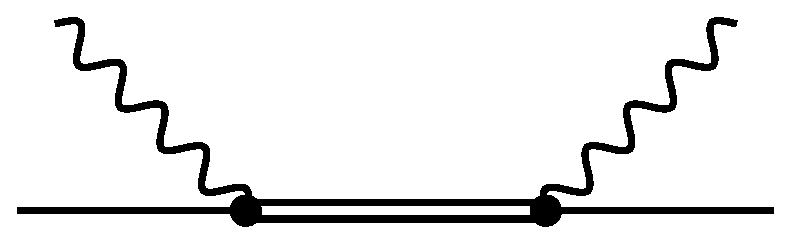
\epsfig{file=DeltaExchange.eps,width=5cm,angle=0}
\caption{$\Delta$-exchange diagram. \label{DeltaExchange}}
\end{figure}

In this section, we give analytical expressions for the  tree-level $\Delta$-exchange contributions, cf.\ Fig.~\ref{DeltaExchange}, to the nucleon polarizabilities and their slopes at $Q^2=0$. Note that the $\Delta$ exchange equally contributions to proton and neutron polarizabilities. The $\gamma^* N \Delta$ vertex follows from the Lagrangian given in \Eqref{gammaNDeltaLag}:
\bea
%\Gamma_{\Delta \rightarrow \gamma N}^{\al \mu}&=&-\sqrt{\frac{3}{2}}\frac{e}{M(M+M_\Delta)}\left\{g_M \gamma^{\al \mu \kappa \lambda}p'_\kappa q_\lambda+g_E(p'\cdot q\, g^{\al \mu}-q^\al p^{\prime\mu})\right.\\
%&&\left.-\frac{g_C}{M_\Delta} \left(q^2 g^{ \al \mu}\slashed{p}'-q^2 p^{\prime\mu} \gamma^\al +p'\cdot q \,q^\mu \gamma^\al-q^\al q^\mu \slashed{p}'\right)\right\}\gamma_5,\qquad\nn\\
\Gamma_{\gamma N \rightarrow \Delta}^{\al \mu}&=&\sqrt{\frac{3}{2}}\frac{e}{M_N M_+}T_3^\dagger\left\{g_M \gamma^{\al \mu \kappa \lambda}p'_\kappa q_\lambda+g_E (p'\cdot q\, g^{\al \mu}-q^\al p^{\prime\mu})\right.\\
&&\left.+\frac{g_C}{M_\Delta} \left(q^2 g^{ \al \mu}\slashed{p}'-q^2 p^{\prime\mu} \gamma^\al +p'\cdot q \,q^\mu \gamma^\al-q^\al q^\mu \slashed{p}'\right)\right\}\gamma_5,\qquad\nn
\eea
with $p+q=p'$, where $p$, $q$ and $p'$ are the momenta of nucleon, photon and Delta, respectively. Here, we use $\varDelta = M_\Delta - M_N$, $M_+=M_\Delta+M_N$, and the couplings are given in Table \ref{tab:constants}.  Remember that for the magnetic coupling, we introduced the following $Q^2$ dependence: $g_M \rightarrow g_M/(1+Q^2/\Lambda^2)^2$.


\bea
\eqlab{alphabetaQ2}
\al_{E1}&=&-\frac{e^2 g_E^2}{2 \pi  M_+^3}\\
\be_{M1}&=&\frac{e^2 g_M^2}{2 \pi  \varDelta  M_+^2}\\
\al_L&=&\frac{e^2 M_\Delta^2}{\pi M_+^3}\left(\frac{ g_E^2}{\varDelta  M_NM_+^2}-\frac{g_C^2}{2 M_\Delta^4}+\frac{ g_E g_C}{M_NM_\Delta^2 M_+}\right)\\
\eea

\bea
\frac{\dd \left[\alpha_{E1}(Q^2)+\beta_{M1}(Q^2)\right]}{\dd Q^2}\Bigg\vert_{Q^2=0}&=&-\frac{e^2}{\pi M_+^2}\left(\frac{g_M^2}{\varDelta^2}\left[\frac{1}{M_+}-\frac{1}{2\varDelta}\right]+\frac{2}{ \Lambda^2 }\frac{g_M^2}{\varDelta}\right.+\frac{g_M g_E}{M_N}\left[\frac{1}{4\varDelta^2}-\frac{1}{\varDelta M_+}\right.\nn\\
&&\left.\left.+\frac{1}{4M_+^2}\right] -\frac{g_E^2}{4M_NM_+}\left[\frac{1}{\varDelta}-\frac{5}{M_+}\right]-\frac{ g_M g_C}{2  \varDelta  M_NM_+}+\frac{g_E g_C}{M_NM_+^2}\right)\qquad\\
\frac{\dd\, \al_L(Q^2)}{\dd Q^2}\Bigg\vert_{Q^2=0}&=&\frac{e^2 M_\Delta^3}{\pi \varDelta M_+^4}\Big(\frac{2g_E^2}{\varDelta^2 M_+^2}\Big[\frac{2}{M_\Delta}-\frac{1}{M_N}\big]-\frac{g_C^2}{ M_\Delta^4}\Big[\frac{1}{M_N}-\frac{3}{2M_\Delta}\Big] \nonumber \\
&&+\frac{g_E g_C}{\varDelta M_\Delta^2 M_+}\Big[\frac{5}{M_\Delta}-\frac{3}{M_N}\Big]\Big)\qquad\\
\eqlab{d2momQ2}
\eea






%\end{widetext}




%\clearpage


%%% FIGURES



%\section{Convergence}



\begin{figure}
\begin{center}
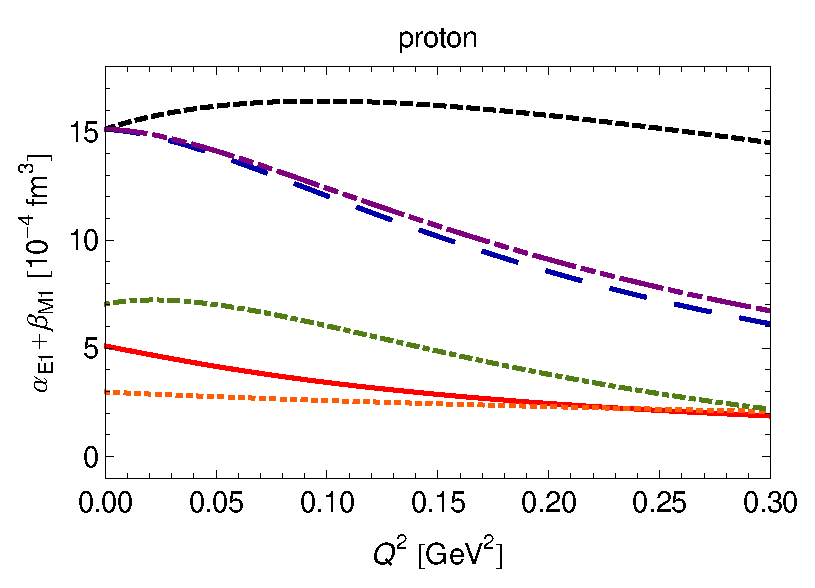
\epsfig{file=alpha+beta_p-orders-Dip.eps,width=6.1cm,angle=0}\hspace{0.5cm}
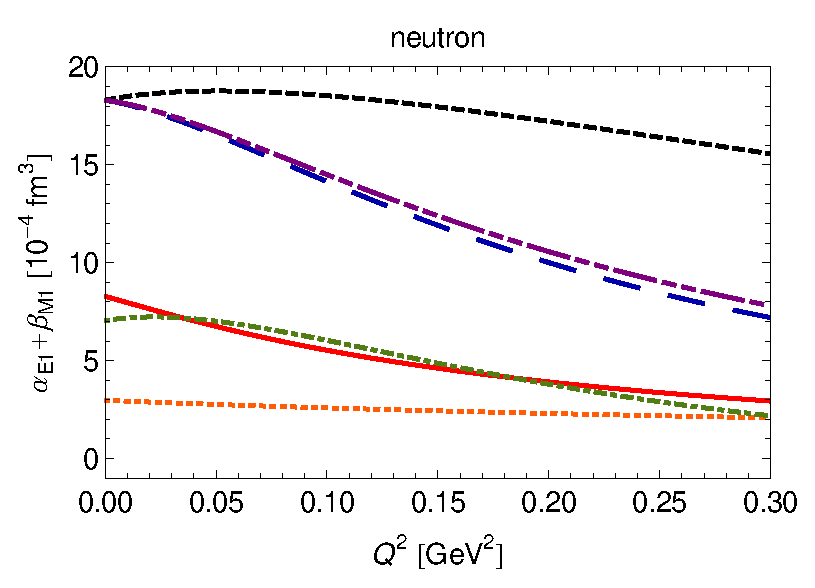
\epsfig{file=alpha+beta_n-orders-Dip.eps,width=6.1cm,angle=0} 
\caption{\small{Contributions of the different orders to the chiral prediction of $[\alpha_{E1}+\beta_{M1}](Q^2)$. Red short-dashed line: $\pi N$-loop contribution, green dot-dashed line: $\Delta$-exchange contribution, orange dotted line: $\pi \Delta$-loop contribution, blue solid line: total result, blue long-dashed line: total result without $g_C$ contribution, purple dot-dot-dashed line: total result without $g_M$ dipole.}\label{Fig:alpha+beta-orders}}
\end{center}
\end{figure}



\begin{figure}
\begin{center}
\epsfig{file=alphaL_p-orders.eps,width=6.1cm,angle=0}\hspace{0.5cm} \epsfig{file=alphaL_n-orders.eps,width=6.1cm,angle=0} 
\caption{Contributions of the different orders to the chiral prediction of $\alpha_{L}(Q^2)$. The legend is the same as in Fig.~\ref{Fig:alpha+beta-orders}. \label{Fig:alphaL-orders}}
\end{center}
\end{figure}



%\begin{widetext}

\begin{figure*}
\begin{center} 
\includegraphics[width=0.75\textwidth]{ProtonSummaryCrossSections}
\caption{Proton photoabsorption cross sections for $\pi N$ (red) and $\pi \Delta$ production (orange) with $Q^2=0$ (solid) and $Q^2=0.1$ GeV$^2$ (dashed for $\pi N$ and dotted for $\pi \Delta$ channel). \label{Fig:ProtonSummaryCrossSections}}
\end{center}
\end{figure*}

\begin{figure*}
\begin{center} 
\includegraphics[width=0.75\textwidth]{NeutronSummaryCrossSections}
\caption{Neutron photoabsorption cross sections for $\pi N$ (red) and $\pi \Delta$ production (orange) with $Q^2=0$ (solid) and $Q^2=0.1$ GeV$^2$ (dashed for $\pi N$ and dotted for $\pi \Delta$ channel). \label{Fig:NeutronSummaryCrossSections}}
\end{center}
\end{figure*}

%\end{widetext}

%\begin{figure}
%\begin{center}
%\epsfig{file=I1p-NoDip.eps,width=8cm,angle=0} \epsfig{file=I1n-NoDip.eps,width=8cm,angle=0} 
%\caption{Comparison of the full result without dipole (red solid line) with the rest of the available $\chi$PT calculations for $I_{1}$. The blue solid line and its band is our total result with dipole, and the blue dashed line is the HB result (Ref.~\cite{Kao:2002cp}) and the grey band is the B$\chi$PT+$\Delta$ result of \cite{Bernard:2012hb}. The data are the same as in Fig~\ref{Fig:I1plot}.\label{Fig:I1-NoDip}}
%\end{center}
%\end{figure}


%\begin{figure}
%\begin{center}
%\epsfig{file=Gamma1p-NoDip.eps,width=8cm,angle=0} \epsfig{file=Gamma1n-NoDip.eps,width=8cm,angle=0} 
%\caption{Comparison of the full result without dipole (red solid line) with the rest of the available $\chi$PT calculations for $\Gamma_{1}$. The blue solid line and its band is our total result with dipole, and the blue dashed line is the HB result (Ref.~\cite{Kao:2002cp}) and the grey band is the B$\chi$PT+$\Delta$ result of \cite{Bernard:2012hb}. The data are the same as in Fig~\ref{Fig:Gamma1plot}.\label{Fig:Gamma1-NoDip}}
%\end{center}
%\end{figure}


%\begin{figure}
%\begin{center}
%\epsfig{file=alpha+beta_p-NoDip.eps,width=8cm,angle=0} \epsfig{file=alpha+beta_n-NoDip.eps,width=8cm,angle=0} 
%\caption{Comparison of the full result without dipole (red solid line) with the rest of the available $\chi$PT calculations for $\alpha+\beta$. The blue solid line and its band is our total result with dipole and the blue dashed line is the leading order result of \cite{Nevado:2007dd}. The data are the same as in Fig~\ref{Fig:alpha+betaplot}.\label{Fig:alpha+beta-NoDip}}
%\end{center}
%\end{figure}

%\begin{figure}
%\begin{center}
%\epsfig{file=IAp-NoDip.eps,width=8cm,angle=0} \epsfig{file=IAn-NoDip.eps,width=8cm,angle=0} 
%\caption{Comparison of the full result without dipole (red solid line) with the rest of the available $\chi$PT calculations for $I_{A}$. The blue solid line and its band is our total result with dipole, and the blue dashed line is the HB result (Ref.~\cite{Kao:2002cp}) and the grey band is the B$\chi$PT+$\Delta$ result of \cite{Bernard:2012hb}. The data are the same as in Fig~\ref{Fig:IAplot}.\label{Fig:IA-NoDip}}
%\end{center}
%\end{figure}

%\begin{figure}
%\begin{center}
%\epsfig{file=d2p-NoDip.eps,width=8cm,angle=0} \epsfig{file=d2n-NoDip.eps,width=8cm,angle=0} 
%\caption{Comparison of the full result without dipole (red solid line) with the rest of the available $\chi$PT calculations for $\bar{d}_{2}$. The blue solid line and its band is our total result with dipole, and the blue dashed line is the HB result (Ref.~\cite{Kao:2002cp}) and the grey band is the B$\chi$PT+$\Delta$ result of \cite{Bernard:2012hb}. The data are the same as in Fig~\ref{Fig:d2plot}.\label{Fig:d2-NoDip}}
%\end{center}
%\end{figure} 

%\begin{figure}
%\begin{center}
%\epsfig{file=deltaLT_p-NoDip.eps,width=8cm,angle=0} \epsfig{file=deltaLT_n-NoDip.eps,width=8cm,angle=0} 
%\caption{Comparison of the full result without dipole (red solid line) with the rest of the available $\chi$PT calculations for $\delta_{LT}$. The blue solid line and its band is our total result with dipole, and the blue dashed line is the HB result (Ref.~\cite{Kao:2002cp}) and the grey band is the B$\chi$PT+$\Delta$ result of \cite{Bernard:2012hb}. The data are the same as in Fig~\ref{Fig:deltaLTplot}.\label{Fig:deltaLT-NoDip}}
%\end{center}
%\end{figure}

%\begin{figure}
%\begin{center}
%\epsfig{file=gamma0_p-NoDip.eps,width=8cm,angle=0} \epsfig{file=gamma0_n-NoDip.eps,width=8cm,angle=0} 
%\caption{Comparison of the full result without dipole (red solid line) with the rest of the available $\chi$PT calculations for $\gamma_0$. The blue solid line and its band is our total result with dipole, the blue dashed line is the HB result (Ref.~\cite{Kao:2002cp}) and the grey band is the B$\chi$PT+$\Delta$ result of \cite{Bernard:2012hb}. The data are the same as in Fig~\ref{Fig:gamma0plot}.\label{Fig:gamma0-NoDip}}
%\end{center}
%\end{figure}

\newpage
\begin{spacing}{0.8}
\small
\bibliographystyle{model1a-num-names}

\bibliography{lowQ}
\end{spacing}


\end{document}